\documentclass[11pt]{article}

    \usepackage[breakable]{tcolorbox}
    \usepackage{parskip} % Stop auto-indenting (to mimic markdown behaviour)
    
    \usepackage{iftex}
    \ifPDFTeX
    	\usepackage[T1]{fontenc}
    	\usepackage{mathpazo}
    \else
    	\usepackage{fontspec}
    \fi

    % Basic figure setup, for now with no caption control since it's done
    % automatically by Pandoc (which extracts ![](path) syntax from Markdown).
    \usepackage{graphicx}
    % Maintain compatibility with old templates. Remove in nbconvert 6.0
    \let\Oldincludegraphics\includegraphics
    % Ensure that by default, figures have no caption (until we provide a
    % proper Figure object with a Caption API and a way to capture that
    % in the conversion process - todo).
    \usepackage{caption}
    \DeclareCaptionFormat{nocaption}{}
    \captionsetup{format=nocaption,aboveskip=0pt,belowskip=0pt}

    \usepackage[Export]{adjustbox} % Used to constrain images to a maximum size
    \adjustboxset{max size={0.9\linewidth}{0.9\paperheight}}
    \usepackage{float}
    \floatplacement{figure}{H} % forces figures to be placed at the correct location
    \usepackage{xcolor} % Allow colors to be defined
    \usepackage{enumerate} % Needed for markdown enumerations to work
    \usepackage{geometry} % Used to adjust the document margins
    \usepackage{amsmath} % Equations
    \usepackage{amssymb} % Equations
    \usepackage{textcomp} % defines textquotesingle
    % Hack from http://tex.stackexchange.com/a/47451/13684:
    \AtBeginDocument{%
        \def\PYZsq{\textquotesingle}% Upright quotes in Pygmentized code
    }
    \usepackage{upquote} % Upright quotes for verbatim code
    \usepackage{eurosym} % defines \euro
    \usepackage[mathletters]{ucs} % Extended unicode (utf-8) support
    \usepackage{fancyvrb} % verbatim replacement that allows latex
    \usepackage{grffile} % extends the file name processing of package graphics 
                         % to support a larger range
    \makeatletter % fix for grffile with XeLaTeX
    \def\Gread@@xetex#1{%
      \IfFileExists{"\Gin@base".bb}%
      {\Gread@eps{\Gin@base.bb}}%
      {\Gread@@xetex@aux#1}%
    }
    \makeatother

    % The hyperref package gives us a pdf with properly built
    % internal navigation ('pdf bookmarks' for the table of contents,
    % internal cross-reference links, web links for URLs, etc.)
    \usepackage{hyperref}
    % The default LaTeX title has an obnoxious amount of whitespace. By default,
    % titling removes some of it. It also provides customization options.
    \usepackage{titling}
    \usepackage{longtable} % longtable support required by pandoc >1.10
    \usepackage{booktabs}  % table support for pandoc > 1.12.2
    \usepackage[inline]{enumitem} % IRkernel/repr support (it uses the enumerate* environment)
    \usepackage[normalem]{ulem} % ulem is needed to support strikethroughs (\sout)
                                % normalem makes italics be italics, not underlines
    \usepackage{mathrsfs}
    

    
    % Colors for the hyperref package
    \definecolor{urlcolor}{rgb}{0,.145,.698}
    \definecolor{linkcolor}{rgb}{.71,0.21,0.01}
    \definecolor{citecolor}{rgb}{.12,.54,.11}

    % ANSI colors
    \definecolor{ansi-black}{HTML}{3E424D}
    \definecolor{ansi-black-intense}{HTML}{282C36}
    \definecolor{ansi-red}{HTML}{E75C58}
    \definecolor{ansi-red-intense}{HTML}{B22B31}
    \definecolor{ansi-green}{HTML}{00A250}
    \definecolor{ansi-green-intense}{HTML}{007427}
    \definecolor{ansi-yellow}{HTML}{DDB62B}
    \definecolor{ansi-yellow-intense}{HTML}{B27D12}
    \definecolor{ansi-blue}{HTML}{208FFB}
    \definecolor{ansi-blue-intense}{HTML}{0065CA}
    \definecolor{ansi-magenta}{HTML}{D160C4}
    \definecolor{ansi-magenta-intense}{HTML}{A03196}
    \definecolor{ansi-cyan}{HTML}{60C6C8}
    \definecolor{ansi-cyan-intense}{HTML}{258F8F}
    \definecolor{ansi-white}{HTML}{C5C1B4}
    \definecolor{ansi-white-intense}{HTML}{A1A6B2}
    \definecolor{ansi-default-inverse-fg}{HTML}{FFFFFF}
    \definecolor{ansi-default-inverse-bg}{HTML}{000000}

    % commands and environments needed by pandoc snippets
    % extracted from the output of `pandoc -s`
    \providecommand{\tightlist}{%
      \setlength{\itemsep}{0pt}\setlength{\parskip}{0pt}}
    \DefineVerbatimEnvironment{Highlighting}{Verbatim}{commandchars=\\\{\}}
    % Add ',fontsize=\small' for more characters per line
    \newenvironment{Shaded}{}{}
    \newcommand{\KeywordTok}[1]{\textcolor[rgb]{0.00,0.44,0.13}{\textbf{{#1}}}}
    \newcommand{\DataTypeTok}[1]{\textcolor[rgb]{0.56,0.13,0.00}{{#1}}}
    \newcommand{\DecValTok}[1]{\textcolor[rgb]{0.25,0.63,0.44}{{#1}}}
    \newcommand{\BaseNTok}[1]{\textcolor[rgb]{0.25,0.63,0.44}{{#1}}}
    \newcommand{\FloatTok}[1]{\textcolor[rgb]{0.25,0.63,0.44}{{#1}}}
    \newcommand{\CharTok}[1]{\textcolor[rgb]{0.25,0.44,0.63}{{#1}}}
    \newcommand{\StringTok}[1]{\textcolor[rgb]{0.25,0.44,0.63}{{#1}}}
    \newcommand{\CommentTok}[1]{\textcolor[rgb]{0.38,0.63,0.69}{\textit{{#1}}}}
    \newcommand{\OtherTok}[1]{\textcolor[rgb]{0.00,0.44,0.13}{{#1}}}
    \newcommand{\AlertTok}[1]{\textcolor[rgb]{1.00,0.00,0.00}{\textbf{{#1}}}}
    \newcommand{\FunctionTok}[1]{\textcolor[rgb]{0.02,0.16,0.49}{{#1}}}
    \newcommand{\RegionMarkerTok}[1]{{#1}}
    \newcommand{\ErrorTok}[1]{\textcolor[rgb]{1.00,0.00,0.00}{\textbf{{#1}}}}
    \newcommand{\NormalTok}[1]{{#1}}
    
    % Additional commands for more recent versions of Pandoc
    \newcommand{\ConstantTok}[1]{\textcolor[rgb]{0.53,0.00,0.00}{{#1}}}
    \newcommand{\SpecialCharTok}[1]{\textcolor[rgb]{0.25,0.44,0.63}{{#1}}}
    \newcommand{\VerbatimStringTok}[1]{\textcolor[rgb]{0.25,0.44,0.63}{{#1}}}
    \newcommand{\SpecialStringTok}[1]{\textcolor[rgb]{0.73,0.40,0.53}{{#1}}}
    \newcommand{\ImportTok}[1]{{#1}}
    \newcommand{\DocumentationTok}[1]{\textcolor[rgb]{0.73,0.13,0.13}{\textit{{#1}}}}
    \newcommand{\AnnotationTok}[1]{\textcolor[rgb]{0.38,0.63,0.69}{\textbf{\textit{{#1}}}}}
    \newcommand{\CommentVarTok}[1]{\textcolor[rgb]{0.38,0.63,0.69}{\textbf{\textit{{#1}}}}}
    \newcommand{\VariableTok}[1]{\textcolor[rgb]{0.10,0.09,0.49}{{#1}}}
    \newcommand{\ControlFlowTok}[1]{\textcolor[rgb]{0.00,0.44,0.13}{\textbf{{#1}}}}
    \newcommand{\OperatorTok}[1]{\textcolor[rgb]{0.40,0.40,0.40}{{#1}}}
    \newcommand{\BuiltInTok}[1]{{#1}}
    \newcommand{\ExtensionTok}[1]{{#1}}
    \newcommand{\PreprocessorTok}[1]{\textcolor[rgb]{0.74,0.48,0.00}{{#1}}}
    \newcommand{\AttributeTok}[1]{\textcolor[rgb]{0.49,0.56,0.16}{{#1}}}
    \newcommand{\InformationTok}[1]{\textcolor[rgb]{0.38,0.63,0.69}{\textbf{\textit{{#1}}}}}
    \newcommand{\WarningTok}[1]{\textcolor[rgb]{0.38,0.63,0.69}{\textbf{\textit{{#1}}}}}
    
    
    % Define a nice break command that doesn't care if a line doesn't already
    % exist.
    \def\br{\hspace*{\fill} \\* }
    % Math Jax compatibility definitions
    \def\gt{>}
    \def\lt{<}
    \let\Oldtex\TeX
    \let\Oldlatex\LaTeX
    \renewcommand{\TeX}{\textrm{\Oldtex}}
    \renewcommand{\LaTeX}{\textrm{\Oldlatex}}
    % Document parameters
    % Document title
    \title{Activity 1}
    
    
    
    
    
% Pygments definitions
\makeatletter
\def\PY@reset{\let\PY@it=\relax \let\PY@bf=\relax%
    \let\PY@ul=\relax \let\PY@tc=\relax%
    \let\PY@bc=\relax \let\PY@ff=\relax}
\def\PY@tok#1{\csname PY@tok@#1\endcsname}
\def\PY@toks#1+{\ifx\relax#1\empty\else%
    \PY@tok{#1}\expandafter\PY@toks\fi}
\def\PY@do#1{\PY@bc{\PY@tc{\PY@ul{%
    \PY@it{\PY@bf{\PY@ff{#1}}}}}}}
\def\PY#1#2{\PY@reset\PY@toks#1+\relax+\PY@do{#2}}

\expandafter\def\csname PY@tok@w\endcsname{\def\PY@tc##1{\textcolor[rgb]{0.73,0.73,0.73}{##1}}}
\expandafter\def\csname PY@tok@c\endcsname{\let\PY@it=\textit\def\PY@tc##1{\textcolor[rgb]{0.25,0.50,0.50}{##1}}}
\expandafter\def\csname PY@tok@cp\endcsname{\def\PY@tc##1{\textcolor[rgb]{0.74,0.48,0.00}{##1}}}
\expandafter\def\csname PY@tok@k\endcsname{\let\PY@bf=\textbf\def\PY@tc##1{\textcolor[rgb]{0.00,0.50,0.00}{##1}}}
\expandafter\def\csname PY@tok@kp\endcsname{\def\PY@tc##1{\textcolor[rgb]{0.00,0.50,0.00}{##1}}}
\expandafter\def\csname PY@tok@kt\endcsname{\def\PY@tc##1{\textcolor[rgb]{0.69,0.00,0.25}{##1}}}
\expandafter\def\csname PY@tok@o\endcsname{\def\PY@tc##1{\textcolor[rgb]{0.40,0.40,0.40}{##1}}}
\expandafter\def\csname PY@tok@ow\endcsname{\let\PY@bf=\textbf\def\PY@tc##1{\textcolor[rgb]{0.67,0.13,1.00}{##1}}}
\expandafter\def\csname PY@tok@nb\endcsname{\def\PY@tc##1{\textcolor[rgb]{0.00,0.50,0.00}{##1}}}
\expandafter\def\csname PY@tok@nf\endcsname{\def\PY@tc##1{\textcolor[rgb]{0.00,0.00,1.00}{##1}}}
\expandafter\def\csname PY@tok@nc\endcsname{\let\PY@bf=\textbf\def\PY@tc##1{\textcolor[rgb]{0.00,0.00,1.00}{##1}}}
\expandafter\def\csname PY@tok@nn\endcsname{\let\PY@bf=\textbf\def\PY@tc##1{\textcolor[rgb]{0.00,0.00,1.00}{##1}}}
\expandafter\def\csname PY@tok@ne\endcsname{\let\PY@bf=\textbf\def\PY@tc##1{\textcolor[rgb]{0.82,0.25,0.23}{##1}}}
\expandafter\def\csname PY@tok@nv\endcsname{\def\PY@tc##1{\textcolor[rgb]{0.10,0.09,0.49}{##1}}}
\expandafter\def\csname PY@tok@no\endcsname{\def\PY@tc##1{\textcolor[rgb]{0.53,0.00,0.00}{##1}}}
\expandafter\def\csname PY@tok@nl\endcsname{\def\PY@tc##1{\textcolor[rgb]{0.63,0.63,0.00}{##1}}}
\expandafter\def\csname PY@tok@ni\endcsname{\let\PY@bf=\textbf\def\PY@tc##1{\textcolor[rgb]{0.60,0.60,0.60}{##1}}}
\expandafter\def\csname PY@tok@na\endcsname{\def\PY@tc##1{\textcolor[rgb]{0.49,0.56,0.16}{##1}}}
\expandafter\def\csname PY@tok@nt\endcsname{\let\PY@bf=\textbf\def\PY@tc##1{\textcolor[rgb]{0.00,0.50,0.00}{##1}}}
\expandafter\def\csname PY@tok@nd\endcsname{\def\PY@tc##1{\textcolor[rgb]{0.67,0.13,1.00}{##1}}}
\expandafter\def\csname PY@tok@s\endcsname{\def\PY@tc##1{\textcolor[rgb]{0.73,0.13,0.13}{##1}}}
\expandafter\def\csname PY@tok@sd\endcsname{\let\PY@it=\textit\def\PY@tc##1{\textcolor[rgb]{0.73,0.13,0.13}{##1}}}
\expandafter\def\csname PY@tok@si\endcsname{\let\PY@bf=\textbf\def\PY@tc##1{\textcolor[rgb]{0.73,0.40,0.53}{##1}}}
\expandafter\def\csname PY@tok@se\endcsname{\let\PY@bf=\textbf\def\PY@tc##1{\textcolor[rgb]{0.73,0.40,0.13}{##1}}}
\expandafter\def\csname PY@tok@sr\endcsname{\def\PY@tc##1{\textcolor[rgb]{0.73,0.40,0.53}{##1}}}
\expandafter\def\csname PY@tok@ss\endcsname{\def\PY@tc##1{\textcolor[rgb]{0.10,0.09,0.49}{##1}}}
\expandafter\def\csname PY@tok@sx\endcsname{\def\PY@tc##1{\textcolor[rgb]{0.00,0.50,0.00}{##1}}}
\expandafter\def\csname PY@tok@m\endcsname{\def\PY@tc##1{\textcolor[rgb]{0.40,0.40,0.40}{##1}}}
\expandafter\def\csname PY@tok@gh\endcsname{\let\PY@bf=\textbf\def\PY@tc##1{\textcolor[rgb]{0.00,0.00,0.50}{##1}}}
\expandafter\def\csname PY@tok@gu\endcsname{\let\PY@bf=\textbf\def\PY@tc##1{\textcolor[rgb]{0.50,0.00,0.50}{##1}}}
\expandafter\def\csname PY@tok@gd\endcsname{\def\PY@tc##1{\textcolor[rgb]{0.63,0.00,0.00}{##1}}}
\expandafter\def\csname PY@tok@gi\endcsname{\def\PY@tc##1{\textcolor[rgb]{0.00,0.63,0.00}{##1}}}
\expandafter\def\csname PY@tok@gr\endcsname{\def\PY@tc##1{\textcolor[rgb]{1.00,0.00,0.00}{##1}}}
\expandafter\def\csname PY@tok@ge\endcsname{\let\PY@it=\textit}
\expandafter\def\csname PY@tok@gs\endcsname{\let\PY@bf=\textbf}
\expandafter\def\csname PY@tok@gp\endcsname{\let\PY@bf=\textbf\def\PY@tc##1{\textcolor[rgb]{0.00,0.00,0.50}{##1}}}
\expandafter\def\csname PY@tok@go\endcsname{\def\PY@tc##1{\textcolor[rgb]{0.53,0.53,0.53}{##1}}}
\expandafter\def\csname PY@tok@gt\endcsname{\def\PY@tc##1{\textcolor[rgb]{0.00,0.27,0.87}{##1}}}
\expandafter\def\csname PY@tok@err\endcsname{\def\PY@bc##1{\setlength{\fboxsep}{0pt}\fcolorbox[rgb]{1.00,0.00,0.00}{1,1,1}{\strut ##1}}}
\expandafter\def\csname PY@tok@kc\endcsname{\let\PY@bf=\textbf\def\PY@tc##1{\textcolor[rgb]{0.00,0.50,0.00}{##1}}}
\expandafter\def\csname PY@tok@kd\endcsname{\let\PY@bf=\textbf\def\PY@tc##1{\textcolor[rgb]{0.00,0.50,0.00}{##1}}}
\expandafter\def\csname PY@tok@kn\endcsname{\let\PY@bf=\textbf\def\PY@tc##1{\textcolor[rgb]{0.00,0.50,0.00}{##1}}}
\expandafter\def\csname PY@tok@kr\endcsname{\let\PY@bf=\textbf\def\PY@tc##1{\textcolor[rgb]{0.00,0.50,0.00}{##1}}}
\expandafter\def\csname PY@tok@bp\endcsname{\def\PY@tc##1{\textcolor[rgb]{0.00,0.50,0.00}{##1}}}
\expandafter\def\csname PY@tok@fm\endcsname{\def\PY@tc##1{\textcolor[rgb]{0.00,0.00,1.00}{##1}}}
\expandafter\def\csname PY@tok@vc\endcsname{\def\PY@tc##1{\textcolor[rgb]{0.10,0.09,0.49}{##1}}}
\expandafter\def\csname PY@tok@vg\endcsname{\def\PY@tc##1{\textcolor[rgb]{0.10,0.09,0.49}{##1}}}
\expandafter\def\csname PY@tok@vi\endcsname{\def\PY@tc##1{\textcolor[rgb]{0.10,0.09,0.49}{##1}}}
\expandafter\def\csname PY@tok@vm\endcsname{\def\PY@tc##1{\textcolor[rgb]{0.10,0.09,0.49}{##1}}}
\expandafter\def\csname PY@tok@sa\endcsname{\def\PY@tc##1{\textcolor[rgb]{0.73,0.13,0.13}{##1}}}
\expandafter\def\csname PY@tok@sb\endcsname{\def\PY@tc##1{\textcolor[rgb]{0.73,0.13,0.13}{##1}}}
\expandafter\def\csname PY@tok@sc\endcsname{\def\PY@tc##1{\textcolor[rgb]{0.73,0.13,0.13}{##1}}}
\expandafter\def\csname PY@tok@dl\endcsname{\def\PY@tc##1{\textcolor[rgb]{0.73,0.13,0.13}{##1}}}
\expandafter\def\csname PY@tok@s2\endcsname{\def\PY@tc##1{\textcolor[rgb]{0.73,0.13,0.13}{##1}}}
\expandafter\def\csname PY@tok@sh\endcsname{\def\PY@tc##1{\textcolor[rgb]{0.73,0.13,0.13}{##1}}}
\expandafter\def\csname PY@tok@s1\endcsname{\def\PY@tc##1{\textcolor[rgb]{0.73,0.13,0.13}{##1}}}
\expandafter\def\csname PY@tok@mb\endcsname{\def\PY@tc##1{\textcolor[rgb]{0.40,0.40,0.40}{##1}}}
\expandafter\def\csname PY@tok@mf\endcsname{\def\PY@tc##1{\textcolor[rgb]{0.40,0.40,0.40}{##1}}}
\expandafter\def\csname PY@tok@mh\endcsname{\def\PY@tc##1{\textcolor[rgb]{0.40,0.40,0.40}{##1}}}
\expandafter\def\csname PY@tok@mi\endcsname{\def\PY@tc##1{\textcolor[rgb]{0.40,0.40,0.40}{##1}}}
\expandafter\def\csname PY@tok@il\endcsname{\def\PY@tc##1{\textcolor[rgb]{0.40,0.40,0.40}{##1}}}
\expandafter\def\csname PY@tok@mo\endcsname{\def\PY@tc##1{\textcolor[rgb]{0.40,0.40,0.40}{##1}}}
\expandafter\def\csname PY@tok@ch\endcsname{\let\PY@it=\textit\def\PY@tc##1{\textcolor[rgb]{0.25,0.50,0.50}{##1}}}
\expandafter\def\csname PY@tok@cm\endcsname{\let\PY@it=\textit\def\PY@tc##1{\textcolor[rgb]{0.25,0.50,0.50}{##1}}}
\expandafter\def\csname PY@tok@cpf\endcsname{\let\PY@it=\textit\def\PY@tc##1{\textcolor[rgb]{0.25,0.50,0.50}{##1}}}
\expandafter\def\csname PY@tok@c1\endcsname{\let\PY@it=\textit\def\PY@tc##1{\textcolor[rgb]{0.25,0.50,0.50}{##1}}}
\expandafter\def\csname PY@tok@cs\endcsname{\let\PY@it=\textit\def\PY@tc##1{\textcolor[rgb]{0.25,0.50,0.50}{##1}}}

\def\PYZbs{\char`\\}
\def\PYZus{\char`\_}
\def\PYZob{\char`\{}
\def\PYZcb{\char`\}}
\def\PYZca{\char`\^}
\def\PYZam{\char`\&}
\def\PYZlt{\char`\<}
\def\PYZgt{\char`\>}
\def\PYZsh{\char`\#}
\def\PYZpc{\char`\%}
\def\PYZdl{\char`\$}
\def\PYZhy{\char`\-}
\def\PYZsq{\char`\'}
\def\PYZdq{\char`\"}
\def\PYZti{\char`\~}
% for compatibility with earlier versions
\def\PYZat{@}
\def\PYZlb{[}
\def\PYZrb{]}
\makeatother


    % For linebreaks inside Verbatim environment from package fancyvrb. 
    \makeatletter
        \newbox\Wrappedcontinuationbox 
        \newbox\Wrappedvisiblespacebox 
        \newcommand*\Wrappedvisiblespace {\textcolor{red}{\textvisiblespace}} 
        \newcommand*\Wrappedcontinuationsymbol {\textcolor{red}{\llap{\tiny$\m@th\hookrightarrow$}}} 
        \newcommand*\Wrappedcontinuationindent {3ex } 
        \newcommand*\Wrappedafterbreak {\kern\Wrappedcontinuationindent\copy\Wrappedcontinuationbox} 
        % Take advantage of the already applied Pygments mark-up to insert 
        % potential linebreaks for TeX processing. 
        %        {, <, #, %, $, ' and ": go to next line. 
        %        _, }, ^, &, >, - and ~: stay at end of broken line. 
        % Use of \textquotesingle for straight quote. 
        \newcommand*\Wrappedbreaksatspecials {% 
            \def\PYGZus{\discretionary{\char`\_}{\Wrappedafterbreak}{\char`\_}}% 
            \def\PYGZob{\discretionary{}{\Wrappedafterbreak\char`\{}{\char`\{}}% 
            \def\PYGZcb{\discretionary{\char`\}}{\Wrappedafterbreak}{\char`\}}}% 
            \def\PYGZca{\discretionary{\char`\^}{\Wrappedafterbreak}{\char`\^}}% 
            \def\PYGZam{\discretionary{\char`\&}{\Wrappedafterbreak}{\char`\&}}% 
            \def\PYGZlt{\discretionary{}{\Wrappedafterbreak\char`\<}{\char`\<}}% 
            \def\PYGZgt{\discretionary{\char`\>}{\Wrappedafterbreak}{\char`\>}}% 
            \def\PYGZsh{\discretionary{}{\Wrappedafterbreak\char`\#}{\char`\#}}% 
            \def\PYGZpc{\discretionary{}{\Wrappedafterbreak\char`\%}{\char`\%}}% 
            \def\PYGZdl{\discretionary{}{\Wrappedafterbreak\char`\$}{\char`\$}}% 
            \def\PYGZhy{\discretionary{\char`\-}{\Wrappedafterbreak}{\char`\-}}% 
            \def\PYGZsq{\discretionary{}{\Wrappedafterbreak\textquotesingle}{\textquotesingle}}% 
            \def\PYGZdq{\discretionary{}{\Wrappedafterbreak\char`\"}{\char`\"}}% 
            \def\PYGZti{\discretionary{\char`\~}{\Wrappedafterbreak}{\char`\~}}% 
        } 
        % Some characters . , ; ? ! / are not pygmentized. 
        % This macro makes them "active" and they will insert potential linebreaks 
        \newcommand*\Wrappedbreaksatpunct {% 
            \lccode`\~`\.\lowercase{\def~}{\discretionary{\hbox{\char`\.}}{\Wrappedafterbreak}{\hbox{\char`\.}}}% 
            \lccode`\~`\,\lowercase{\def~}{\discretionary{\hbox{\char`\,}}{\Wrappedafterbreak}{\hbox{\char`\,}}}% 
            \lccode`\~`\;\lowercase{\def~}{\discretionary{\hbox{\char`\;}}{\Wrappedafterbreak}{\hbox{\char`\;}}}% 
            \lccode`\~`\:\lowercase{\def~}{\discretionary{\hbox{\char`\:}}{\Wrappedafterbreak}{\hbox{\char`\:}}}% 
            \lccode`\~`\?\lowercase{\def~}{\discretionary{\hbox{\char`\?}}{\Wrappedafterbreak}{\hbox{\char`\?}}}% 
            \lccode`\~`\!\lowercase{\def~}{\discretionary{\hbox{\char`\!}}{\Wrappedafterbreak}{\hbox{\char`\!}}}% 
            \lccode`\~`\/\lowercase{\def~}{\discretionary{\hbox{\char`\/}}{\Wrappedafterbreak}{\hbox{\char`\/}}}% 
            \catcode`\.\active
            \catcode`\,\active 
            \catcode`\;\active
            \catcode`\:\active
            \catcode`\?\active
            \catcode`\!\active
            \catcode`\/\active 
            \lccode`\~`\~ 	
        }
    \makeatother

    \let\OriginalVerbatim=\Verbatim
    \makeatletter
    \renewcommand{\Verbatim}[1][1]{%
        %\parskip\z@skip
        \sbox\Wrappedcontinuationbox {\Wrappedcontinuationsymbol}%
        \sbox\Wrappedvisiblespacebox {\FV@SetupFont\Wrappedvisiblespace}%
        \def\FancyVerbFormatLine ##1{\hsize\linewidth
            \vtop{\raggedright\hyphenpenalty\z@\exhyphenpenalty\z@
                \doublehyphendemerits\z@\finalhyphendemerits\z@
                \strut ##1\strut}%
        }%
        % If the linebreak is at a space, the latter will be displayed as visible
        % space at end of first line, and a continuation symbol starts next line.
        % Stretch/shrink are however usually zero for typewriter font.
        \def\FV@Space {%
            \nobreak\hskip\z@ plus\fontdimen3\font minus\fontdimen4\font
            \discretionary{\copy\Wrappedvisiblespacebox}{\Wrappedafterbreak}
            {\kern\fontdimen2\font}%
        }%
        
        % Allow breaks at special characters using \PYG... macros.
        \Wrappedbreaksatspecials
        % Breaks at punctuation characters . , ; ? ! and / need catcode=\active 	
        \OriginalVerbatim[#1,codes*=\Wrappedbreaksatpunct]%
    }
    \makeatother

    % Exact colors from NB
    \definecolor{incolor}{HTML}{303F9F}
    \definecolor{outcolor}{HTML}{D84315}
    \definecolor{cellborder}{HTML}{CFCFCF}
    \definecolor{cellbackground}{HTML}{F7F7F7}
    
    % prompt
    \makeatletter
    \newcommand{\boxspacing}{\kern\kvtcb@left@rule\kern\kvtcb@boxsep}
    \makeatother
    \newcommand{\prompt}[4]{
        \ttfamily\llap{{\color{#2}[#3]:\hspace{3pt}#4}}\vspace{-\baselineskip}
    }
    

    
    % Prevent overflowing lines due to hard-to-break entities
    \sloppy 
    % Setup hyperref package
    \hypersetup{
      breaklinks=true,  % so long urls are correctly broken across lines
      colorlinks=true,
      urlcolor=urlcolor,
      linkcolor=linkcolor,
      citecolor=citecolor,
      }
    % Slightly bigger margins than the latex defaults
    
    \geometry{verbose,tmargin=1in,bmargin=1in,lmargin=1in,rmargin=1in}
    
    

\begin{document}
    
    \maketitle
    
    

    
    \hypertarget{activity-1}{%
\section{Activity 1}\label{activity-1}}

Class activity. Solve for current.

    \hypertarget{problem-1}{%
\subsubsection{Problem 1}\label{problem-1}}

\begin{figure}
\centering
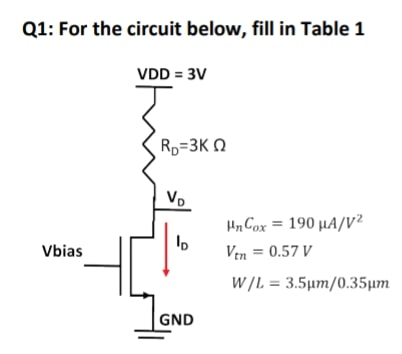
\includegraphics{./image/act1_p1.jpg}
\caption{Problem-1}
\end{figure}

    \begin{longtable}[]{@{}llll@{}}
\toprule
\(V_{bias}\) & MOSFET Operation Mode & \(I_D\) (mA) & \(V_D\)
(V)\tabularnewline
\midrule
\endhead
0.5 & OFF & 0 & 3\tabularnewline
1.0 & SAT & .175 & 2.47\tabularnewline
1.2 & SAT & .377 & 1.87\tabularnewline
1.5 & SAT & .77 & .69\tabularnewline
2.0 & LINEAR & .87 & .37\tabularnewline
3.0 & LINEAR & .93 & .21\tabularnewline
\bottomrule
\end{longtable}

    \begin{tcolorbox}[breakable, size=fbox, boxrule=1pt, pad at break*=1mm,colback=cellbackground, colframe=cellborder]
\prompt{In}{incolor}{49}{\boxspacing}
\begin{Verbatim}[commandchars=\\\{\}]
\PY{k+kn}{import} \PY{n+nn}{cmath}

\PY{c+c1}{\PYZsh{} saturation}
\PY{k}{def} \PY{n+nf}{saturation\PYZus{}current} \PY{p}{(}\PY{n}{VGS}\PY{p}{,} \PY{n}{VTH}\PY{p}{,} \PY{n}{K}\PY{p}{,}\PY{n}{fet\PYZus{}mode}\PY{o}{=}\PY{l+s+s2}{\PYZdq{}}\PY{l+s+s2}{\PYZdq{}}\PY{p}{)}\PY{p}{:}
    \PY{k}{if} \PY{n}{fet\PYZus{}mode}\PY{o}{==}\PY{l+s+s2}{\PYZdq{}}\PY{l+s+s2}{sat}\PY{l+s+s2}{\PYZdq{}}\PY{p}{:}
        \PY{n+nb}{print}\PY{p}{(}\PY{l+s+s2}{\PYZdq{}}\PY{l+s+s2}{The saturation current is: }\PY{l+s+si}{\PYZob{}\PYZcb{}}\PY{l+s+s2}{ mA}\PY{l+s+s2}{\PYZdq{}}\PY{o}{.}\PY{n}{format}\PY{p}{(}\PY{l+m+mf}{0.5}\PY{o}{*}\PY{n}{K}\PY{o}{*}\PY{p}{(}\PY{n}{VGS}\PY{o}{\PYZhy{}}\PY{n}{VTH}\PY{p}{)}\PY{o}{*}\PY{o}{*}\PY{l+m+mi}{2}\PY{o}{*}\PY{l+m+mi}{10}\PY{o}{*}\PY{o}{*}\PY{l+m+mi}{3}\PY{p}{)}\PY{p}{)}
        \PY{k}{return} \PY{l+m+mf}{0.5}\PY{o}{*}\PY{n}{K}\PY{o}{*}\PY{p}{(}\PY{n}{VGS}\PY{o}{\PYZhy{}}\PY{n}{VTH}\PY{p}{)}\PY{o}{*}\PY{o}{*}\PY{l+m+mi}{2}
    \PY{k}{return} \PY{k+kc}{None}
\PY{k}{def} \PY{n+nf}{drain\PYZus{}voltage} \PY{p}{(}\PY{n}{VCC}\PY{o}{=}\PY{k+kc}{None}\PY{p}{,} \PY{n}{ID}\PY{o}{=}\PY{k+kc}{None}\PY{p}{,} \PY{n}{RD}\PY{o}{=}\PY{k+kc}{None}\PY{p}{,} \PY{n}{VGS}\PY{o}{=}\PY{k+kc}{None}\PY{p}{,} \PY{n}{VTH}\PY{o}{=}\PY{k+kc}{None}\PY{p}{,} \PY{n}{VDS}\PY{o}{=}\PY{k+kc}{None}\PY{p}{,} \PY{n}{fet\PYZus{}mode}\PY{o}{=}\PY{l+s+s1}{\PYZsq{}}\PY{l+s+s1}{\PYZsq{}}\PY{p}{)}\PY{p}{:}
    \PY{k}{if} \PY{n}{fet\PYZus{}mode}\PY{o}{==}\PY{l+s+s2}{\PYZdq{}}\PY{l+s+s2}{sat}\PY{l+s+s2}{\PYZdq{}}\PY{p}{:}
        \PY{n}{VDS} \PY{o}{=} \PY{n+nb}{round}\PY{p}{(}\PY{n}{VCC}\PY{o}{\PYZhy{}}\PY{n}{ID}\PY{o}{*}\PY{n}{RD}\PY{p}{,}\PY{l+m+mi}{3}\PY{p}{)}
        \PY{n}{mode\PYZus{}true} \PY{o}{=} \PY{n}{VDS} \PY{o}{\PYZgt{}} \PY{p}{(}\PY{n}{VGS}\PY{o}{\PYZhy{}}\PY{n}{VTH}\PY{p}{)}
        \PY{n+nb}{print}\PY{p}{(}\PY{l+s+s2}{\PYZdq{}}\PY{l+s+s2}{VDS = }\PY{l+s+si}{\PYZob{}\PYZcb{}}\PY{l+s+s2}{ V, the assumption is }\PY{l+s+si}{\PYZob{}\PYZcb{}}\PY{l+s+s2}{.}\PY{l+s+s2}{\PYZdq{}}\PY{o}{.}\PY{n}{format}\PY{p}{(}\PY{n}{VDS}\PY{p}{,} \PY{n}{mode\PYZus{}true}\PY{p}{)}\PY{p}{)}
        \PY{k}{return} \PY{n}{VDS}
    \PY{k}{elif} \PY{n}{fet\PYZus{}mode}\PY{o}{==}\PY{l+s+s1}{\PYZsq{}}\PY{l+s+s1}{triode}\PY{l+s+s1}{\PYZsq{}}\PY{p}{:}
        \PY{n}{mode\PYZus{}true} \PY{o}{=} \PY{n}{VDS} \PY{o}{\PYZlt{}} \PY{p}{(}\PY{n}{VGS}\PY{o}{\PYZhy{}}\PY{n}{VTH}\PY{p}{)}
        \PY{n+nb}{print}\PY{p}{(}\PY{l+s+s2}{\PYZdq{}}\PY{l+s+s2}{VDS = }\PY{l+s+si}{\PYZob{}\PYZcb{}}\PY{l+s+s2}{ V, the assumption is }\PY{l+s+si}{\PYZob{}\PYZcb{}}\PY{l+s+s2}{.}\PY{l+s+s2}{\PYZdq{}}\PY{o}{.}\PY{n}{format}\PY{p}{(}\PY{n}{VDS}\PY{p}{,} \PY{n}{mode\PYZus{}true}\PY{p}{)}\PY{p}{)}
        \PY{k}{return} \PY{n}{VDS}
    \PY{k}{return} \PY{k+kc}{None}

\PY{c+c1}{\PYZsh{} Triode}
\PY{k}{def} \PY{n+nf}{quadratic\PYZus{}formula} \PY{p}{(}\PY{n}{a}\PY{p}{,}\PY{n}{b}\PY{p}{,}\PY{n}{c}\PY{p}{)}\PY{p}{:}
    \PY{n}{d} \PY{o}{=} \PY{p}{(}\PY{n}{b}\PY{o}{*}\PY{o}{*}\PY{l+m+mi}{2}\PY{p}{)} \PY{o}{\PYZhy{}} \PY{p}{(}\PY{l+m+mi}{4}\PY{o}{*}\PY{n}{a}\PY{o}{*}\PY{n}{c}\PY{p}{)}  
    \PY{n}{sol1} \PY{o}{=} \PY{p}{(}\PY{o}{\PYZhy{}}\PY{n}{b}\PY{o}{\PYZhy{}}\PY{n}{cmath}\PY{o}{.}\PY{n}{sqrt}\PY{p}{(}\PY{n}{d}\PY{p}{)}\PY{p}{)}\PY{o}{/}\PY{p}{(}\PY{l+m+mi}{2}\PY{o}{*}\PY{n}{a}\PY{p}{)}  
    \PY{n}{sol2} \PY{o}{=} \PY{p}{(}\PY{o}{\PYZhy{}}\PY{n}{b}\PY{o}{+}\PY{n}{cmath}\PY{o}{.}\PY{n}{sqrt}\PY{p}{(}\PY{n}{d}\PY{p}{)}\PY{p}{)}\PY{o}{/}\PY{p}{(}\PY{l+m+mi}{2}\PY{o}{*}\PY{n}{a}\PY{p}{)}  
    \PY{n+nb}{print}\PY{p}{(}\PY{l+s+s1}{\PYZsq{}}\PY{l+s+s1}{The solution are }\PY{l+s+si}{\PYZob{}0\PYZcb{}}\PY{l+s+s1}{ and }\PY{l+s+si}{\PYZob{}1\PYZcb{}}\PY{l+s+s1}{\PYZsq{}}\PY{o}{.}\PY{n}{format}\PY{p}{(}\PY{n}{sol1}\PY{p}{,}\PY{n}{sol2}\PY{p}{)}\PY{p}{)}
    \PY{k}{return} \PY{p}{[}\PY{n}{sol1}\PY{p}{,} \PY{n}{sol2}\PY{p}{]}
\PY{k}{def} \PY{n+nf}{current\PYZus{}post\PYZus{}quad} \PY{p}{(}\PY{n}{VCC}\PY{p}{,} \PY{n}{VDS}\PY{p}{,} \PY{n}{RD}\PY{p}{)}\PY{p}{:}
    \PY{n}{ID} \PY{o}{=} \PY{p}{(}\PY{n}{VCC}\PY{o}{\PYZhy{}}\PY{n}{VDS}\PY{p}{)}\PY{o}{/}\PY{n}{RD}
    \PY{n+nb}{print}\PY{p}{(}\PY{l+s+s1}{\PYZsq{}}\PY{l+s+s1}{ID = }\PY{l+s+si}{\PYZob{}\PYZcb{}}\PY{l+s+s1}{ A}\PY{l+s+s1}{\PYZsq{}}\PY{o}{.}\PY{n}{format}\PY{p}{(}\PY{p}{(}\PY{n}{VCC}\PY{o}{\PYZhy{}}\PY{n}{VDS}\PY{p}{)}\PY{o}{/}\PY{n}{RD}\PY{p}{)}\PY{p}{)}
    \PY{k}{return} \PY{n}{ID}
\end{Verbatim}
\end{tcolorbox}

    \begin{tcolorbox}[breakable, size=fbox, boxrule=1pt, pad at break*=1mm,colback=cellbackground, colframe=cellborder]
\prompt{In}{incolor}{50}{\boxspacing}
\begin{Verbatim}[commandchars=\\\{\}]
\PY{n}{W} \PY{o}{=} \PY{l+m+mf}{3.5}
\PY{n}{L} \PY{o}{=} \PY{l+m+mf}{0.35}
\PY{n}{K\PYZus{}prime} \PY{o}{=} \PY{l+m+mi}{190}\PY{o}{*}\PY{l+m+mi}{10}\PY{o}{*}\PY{o}{*}\PY{p}{(}\PY{o}{\PYZhy{}}\PY{l+m+mi}{6}\PY{p}{)}
\PY{n}{Kn} \PY{o}{=} \PY{n}{W}\PY{o}{/}\PY{n}{L}\PY{o}{*}\PY{n}{K\PYZus{}prime}
\PY{n}{VGS} \PY{o}{=} \PY{l+m+mi}{1}
\PY{n}{VTH} \PY{o}{=} \PY{l+m+mf}{0.57}
\PY{n}{ID} \PY{o}{=} \PY{n}{saturation\PYZus{}current}\PY{p}{(}\PY{n}{VGS}\PY{p}{,}\PY{n}{VTH}\PY{p}{,}\PY{n}{Kn}\PY{p}{,}\PY{n}{fet\PYZus{}mode}\PY{o}{=}\PY{l+s+s1}{\PYZsq{}}\PY{l+s+s1}{sat}\PY{l+s+s1}{\PYZsq{}}\PY{p}{)}
\PY{n}{VCC} \PY{o}{=} \PY{l+m+mi}{3}
\PY{n}{RD}\PY{o}{=}\PY{l+m+mi}{3000}
\PY{c+c1}{\PYZsh{}verification}
\PY{n}{drain\PYZus{}voltage} \PY{p}{(}\PY{n}{VCC}\PY{o}{=}\PY{n}{VCC}\PY{p}{,} \PY{n}{ID}\PY{o}{=}\PY{n}{ID}\PY{p}{,} \PY{n}{RD}\PY{o}{=}\PY{n}{RD}\PY{p}{,} \PY{n}{VGS}\PY{o}{=}\PY{n}{VGS}\PY{p}{,}\PY{n}{VTH}\PY{o}{=}\PY{n}{VTH}\PY{p}{,} \PY{n}{fet\PYZus{}mode}\PY{o}{=}\PY{l+s+s1}{\PYZsq{}}\PY{l+s+s1}{sat}\PY{l+s+s1}{\PYZsq{}}\PY{p}{)}
\end{Verbatim}
\end{tcolorbox}

    \begin{Verbatim}[commandchars=\\\{\}]
The saturation current is: 0.175655 mA
VDS = 2.473 V, the assumption is True.
    \end{Verbatim}

            \begin{tcolorbox}[breakable, size=fbox, boxrule=.5pt, pad at break*=1mm, opacityfill=0]
\prompt{Out}{outcolor}{50}{\boxspacing}
\begin{Verbatim}[commandchars=\\\{\}]
2.473
\end{Verbatim}
\end{tcolorbox}
        
    \begin{tcolorbox}[breakable, size=fbox, boxrule=1pt, pad at break*=1mm,colback=cellbackground, colframe=cellborder]
\prompt{In}{incolor}{51}{\boxspacing}
\begin{Verbatim}[commandchars=\\\{\}]
\PY{n}{W} \PY{o}{=} \PY{l+m+mf}{3.5}
\PY{n}{L} \PY{o}{=} \PY{l+m+mf}{0.35}
\PY{n}{K\PYZus{}prime} \PY{o}{=} \PY{l+m+mi}{190}\PY{o}{*}\PY{l+m+mi}{10}\PY{o}{*}\PY{o}{*}\PY{p}{(}\PY{o}{\PYZhy{}}\PY{l+m+mi}{6}\PY{p}{)}
\PY{n}{Kn} \PY{o}{=} \PY{n}{W}\PY{o}{/}\PY{n}{L}\PY{o}{*}\PY{n}{K\PYZus{}prime}
\PY{n}{VGS} \PY{o}{=} \PY{l+m+mf}{1.2}
\PY{n}{VTH} \PY{o}{=} \PY{l+m+mf}{0.57}
\PY{n}{ID} \PY{o}{=} \PY{n}{saturation\PYZus{}current}\PY{p}{(}\PY{n}{VGS}\PY{p}{,}\PY{n}{VTH}\PY{p}{,}\PY{n}{Kn}\PY{p}{,}\PY{n}{fet\PYZus{}mode}\PY{o}{=}\PY{l+s+s1}{\PYZsq{}}\PY{l+s+s1}{sat}\PY{l+s+s1}{\PYZsq{}}\PY{p}{)}
\PY{n}{VCC} \PY{o}{=} \PY{l+m+mi}{3}
\PY{n}{RD}\PY{o}{=}\PY{l+m+mi}{3000}
\PY{c+c1}{\PYZsh{}verification}
\PY{n}{drain\PYZus{}voltage} \PY{p}{(}\PY{n}{VCC}\PY{o}{=}\PY{n}{VCC}\PY{p}{,} \PY{n}{ID}\PY{o}{=}\PY{n}{ID}\PY{p}{,} \PY{n}{RD}\PY{o}{=}\PY{n}{RD}\PY{p}{,} \PY{n}{VGS}\PY{o}{=}\PY{n}{VGS}\PY{p}{,}\PY{n}{VTH}\PY{o}{=}\PY{n}{VTH}\PY{p}{,} \PY{n}{fet\PYZus{}mode}\PY{o}{=}\PY{l+s+s1}{\PYZsq{}}\PY{l+s+s1}{sat}\PY{l+s+s1}{\PYZsq{}}\PY{p}{)}
\end{Verbatim}
\end{tcolorbox}

    \begin{Verbatim}[commandchars=\\\{\}]
The saturation current is: 0.377055 mA
VDS = 1.869 V, the assumption is True.
    \end{Verbatim}

            \begin{tcolorbox}[breakable, size=fbox, boxrule=.5pt, pad at break*=1mm, opacityfill=0]
\prompt{Out}{outcolor}{51}{\boxspacing}
\begin{Verbatim}[commandchars=\\\{\}]
1.869
\end{Verbatim}
\end{tcolorbox}
        
    \begin{tcolorbox}[breakable, size=fbox, boxrule=1pt, pad at break*=1mm,colback=cellbackground, colframe=cellborder]
\prompt{In}{incolor}{52}{\boxspacing}
\begin{Verbatim}[commandchars=\\\{\}]
\PY{n}{W} \PY{o}{=} \PY{l+m+mf}{3.5}
\PY{n}{L} \PY{o}{=} \PY{l+m+mf}{0.35}
\PY{n}{K\PYZus{}prime} \PY{o}{=} \PY{l+m+mi}{190}\PY{o}{*}\PY{l+m+mi}{10}\PY{o}{*}\PY{o}{*}\PY{p}{(}\PY{o}{\PYZhy{}}\PY{l+m+mi}{6}\PY{p}{)}
\PY{n}{Kn} \PY{o}{=} \PY{n}{W}\PY{o}{/}\PY{n}{L}\PY{o}{*}\PY{n}{K\PYZus{}prime}
\PY{n}{VGS} \PY{o}{=} \PY{l+m+mf}{1.5}
\PY{n}{VTH} \PY{o}{=} \PY{l+m+mf}{0.57}
\PY{n}{ID} \PY{o}{=} \PY{n}{saturation\PYZus{}current}\PY{p}{(}\PY{n}{VGS}\PY{p}{,}\PY{n}{VTH}\PY{p}{,}\PY{n}{Kn}\PY{p}{,}\PY{n}{fet\PYZus{}mode}\PY{o}{=}\PY{l+s+s1}{\PYZsq{}}\PY{l+s+s1}{sat}\PY{l+s+s1}{\PYZsq{}}\PY{p}{)}
\PY{n}{VCC} \PY{o}{=} \PY{l+m+mi}{3}
\PY{n}{RD}\PY{o}{=}\PY{l+m+mi}{3000}
\PY{c+c1}{\PYZsh{}verification}
\PY{n}{drain\PYZus{}voltage} \PY{p}{(}\PY{n}{VCC}\PY{o}{=}\PY{n}{VCC}\PY{p}{,} \PY{n}{ID}\PY{o}{=}\PY{n}{ID}\PY{p}{,} \PY{n}{RD}\PY{o}{=}\PY{n}{RD}\PY{p}{,} \PY{n}{VGS}\PY{o}{=}\PY{n}{VGS}\PY{p}{,}\PY{n}{VTH}\PY{o}{=}\PY{n}{VTH}\PY{p}{,} \PY{n}{fet\PYZus{}mode}\PY{o}{=}\PY{l+s+s1}{\PYZsq{}}\PY{l+s+s1}{sat}\PY{l+s+s1}{\PYZsq{}}\PY{p}{)}

\PY{c+c1}{\PYZsh{} verification fail \PYZhy{}\PYZgt{} so it\PYZsq{}s triode}
\PY{c+c1}{\PYZsh{} VDS}
\PY{n}{a} \PY{o}{=} \PY{n}{Kn}\PY{o}{/}\PY{l+m+mi}{2}
\PY{n}{b} \PY{o}{=} \PY{o}{\PYZhy{}}\PY{l+m+mi}{1}\PY{o}{*}\PY{p}{(}\PY{l+m+mi}{1}\PY{o}{/}\PY{n}{RD}\PY{o}{+}\PY{n}{Kn}\PY{o}{*}\PY{p}{(}\PY{n}{VGS}\PY{o}{\PYZhy{}}\PY{n}{VTH}\PY{p}{)}\PY{p}{)}
\PY{n}{c} \PY{o}{=} \PY{n}{VCC}\PY{o}{/}\PY{n}{RD}
\PY{n}{Vd1}\PY{p}{,} \PY{n}{Vd2} \PY{o}{=} \PY{n}{quadratic\PYZus{}formula}\PY{p}{(}\PY{n}{a}\PY{o}{=}\PY{n}{a}\PY{p}{,}\PY{n}{b}\PY{o}{=}\PY{n}{b}\PY{p}{,}\PY{n}{c}\PY{o}{=}\PY{n}{c}\PY{p}{)}
\PY{n}{VDS} \PY{o}{=} \PY{n+nb}{min}\PY{p}{(}\PY{n+nb}{abs}\PY{p}{(}\PY{n}{Vd1}\PY{p}{)}\PY{p}{,}\PY{n+nb}{abs}\PY{p}{(}\PY{n}{Vd2}\PY{p}{)}\PY{p}{)}
\PY{n+nb}{print}\PY{p}{(}\PY{l+s+s1}{\PYZsq{}}\PY{l+s+s1}{The valid VDS here is: }\PY{l+s+si}{\PYZob{}\PYZcb{}}\PY{l+s+s1}{ V}\PY{l+s+s1}{\PYZsq{}}\PY{o}{.}\PY{n}{format}\PY{p}{(}\PY{n}{VDS}\PY{p}{)}\PY{p}{)}
\PY{c+c1}{\PYZsh{} ID}
\PY{n}{ID} \PY{o}{=} \PY{n}{current\PYZus{}post\PYZus{}quad}\PY{p}{(}\PY{n}{VCC}\PY{o}{=}\PY{n}{VCC}\PY{p}{,} \PY{n}{VDS}\PY{o}{=}\PY{n}{VDS}\PY{p}{,} \PY{n}{RD}\PY{o}{=}\PY{n}{RD}\PY{p}{)}
\end{Verbatim}
\end{tcolorbox}

    \begin{Verbatim}[commandchars=\\\{\}]
The saturation current is: 0.821655 mA
VDS = 0.535 V, the assumption is False.
The solution are (0.6939013422053886+0j) and (1.5169758507770679+0j)
The valid VDS here is: 0.6939013422053886 V
ID = 0.0007686995525982037 A
    \end{Verbatim}

    \begin{tcolorbox}[breakable, size=fbox, boxrule=1pt, pad at break*=1mm,colback=cellbackground, colframe=cellborder]
\prompt{In}{incolor}{53}{\boxspacing}
\begin{Verbatim}[commandchars=\\\{\}]
\PY{c+c1}{\PYZsh{} input parameter}
\PY{n}{VCC} \PY{o}{=} \PY{l+m+mi}{3}
\PY{n}{RD}\PY{o}{=}\PY{l+m+mi}{3000}
\PY{n}{W} \PY{o}{=} \PY{l+m+mf}{3.5}
\PY{n}{L} \PY{o}{=} \PY{l+m+mf}{0.35}
\PY{n}{K\PYZus{}prime} \PY{o}{=} \PY{l+m+mi}{190}\PY{o}{*}\PY{l+m+mi}{10}\PY{o}{*}\PY{o}{*}\PY{p}{(}\PY{o}{\PYZhy{}}\PY{l+m+mi}{6}\PY{p}{)}
\PY{n}{Kn} \PY{o}{=} \PY{n}{W}\PY{o}{/}\PY{n}{L}\PY{o}{*}\PY{n}{K\PYZus{}prime}
\PY{n}{VGS} \PY{o}{=} \PY{l+m+mi}{2}
\PY{n}{VTH} \PY{o}{=} \PY{l+m+mf}{0.57}

\PY{c+c1}{\PYZsh{} assumption 1: saturation}
\PY{n}{ID} \PY{o}{=} \PY{n}{saturation\PYZus{}current}\PY{p}{(}\PY{n}{VGS}\PY{p}{,}\PY{n}{VTH}\PY{p}{,}\PY{n}{Kn}\PY{p}{,}\PY{n}{fet\PYZus{}mode}\PY{o}{=}\PY{l+s+s1}{\PYZsq{}}\PY{l+s+s1}{sat}\PY{l+s+s1}{\PYZsq{}}\PY{p}{)}
\PY{c+c1}{\PYZsh{} verification for saturation}
\PY{n}{drain\PYZus{}voltage} \PY{p}{(}\PY{n}{VCC}\PY{o}{=}\PY{n}{VCC}\PY{p}{,} \PY{n}{ID}\PY{o}{=}\PY{n}{ID}\PY{p}{,} \PY{n}{RD}\PY{o}{=}\PY{n}{RD}\PY{p}{,} \PY{n}{VGS}\PY{o}{=}\PY{n}{VGS}\PY{p}{,}\PY{n}{VTH}\PY{o}{=}\PY{n}{VTH}\PY{p}{,} \PY{n}{fet\PYZus{}mode}\PY{o}{=}\PY{l+s+s1}{\PYZsq{}}\PY{l+s+s1}{sat}\PY{l+s+s1}{\PYZsq{}}\PY{p}{)}

\PY{c+c1}{\PYZsh{} assumption 2: triode}
\PY{c+c1}{\PYZsh{} Solving for VDS}
\PY{n}{a} \PY{o}{=} \PY{n}{Kn}\PY{o}{/}\PY{l+m+mi}{2}
\PY{n}{b} \PY{o}{=} \PY{o}{\PYZhy{}}\PY{l+m+mi}{1}\PY{o}{*}\PY{p}{(}\PY{l+m+mi}{1}\PY{o}{/}\PY{n}{RD}\PY{o}{+}\PY{n}{Kn}\PY{o}{*}\PY{p}{(}\PY{n}{VGS}\PY{o}{\PYZhy{}}\PY{n}{VTH}\PY{p}{)}\PY{p}{)}
\PY{n}{c} \PY{o}{=} \PY{n}{VCC}\PY{o}{/}\PY{n}{RD}
\PY{n}{Vd1}\PY{p}{,} \PY{n}{Vd2} \PY{o}{=} \PY{n}{quadratic\PYZus{}formula}\PY{p}{(}\PY{n}{a}\PY{o}{=}\PY{n}{a}\PY{p}{,}\PY{n}{b}\PY{o}{=}\PY{n}{b}\PY{p}{,}\PY{n}{c}\PY{o}{=}\PY{n}{c}\PY{p}{)}
\PY{n}{VDS} \PY{o}{=} \PY{n+nb}{min}\PY{p}{(}\PY{n+nb}{abs}\PY{p}{(}\PY{n}{Vd1}\PY{p}{)}\PY{p}{,}\PY{n+nb}{abs}\PY{p}{(}\PY{n}{Vd2}\PY{p}{)}\PY{p}{)}
\PY{n+nb}{print}\PY{p}{(}\PY{l+s+s1}{\PYZsq{}}\PY{l+s+s1}{The valid VDS here is: }\PY{l+s+si}{\PYZob{}\PYZcb{}}\PY{l+s+s1}{ V}\PY{l+s+s1}{\PYZsq{}}\PY{o}{.}\PY{n}{format}\PY{p}{(}\PY{n}{VDS}\PY{p}{)}\PY{p}{)}
\PY{c+c1}{\PYZsh{} Solving for ID}
\PY{n}{ID} \PY{o}{=} \PY{n}{current\PYZus{}post\PYZus{}quad}\PY{p}{(}\PY{n}{VCC}\PY{o}{=}\PY{n}{VCC}\PY{p}{,} \PY{n}{VDS}\PY{o}{=}\PY{n}{VDS}\PY{p}{,} \PY{n}{RD}\PY{o}{=}\PY{n}{RD}\PY{p}{)}
\PY{c+c1}{\PYZsh{} verification for triode}
\PY{n}{VDS} \PY{o}{=} \PY{n}{drain\PYZus{}voltage}\PY{p}{(}\PY{n}{VDS}\PY{o}{=}\PY{n}{VDS}\PY{p}{,} \PY{n}{VGS}\PY{o}{=}\PY{n}{VGS}\PY{p}{,} \PY{n}{VTH}\PY{o}{=}\PY{n}{VTH}\PY{p}{,} \PY{n}{fet\PYZus{}mode}\PY{o}{=}\PY{l+s+s2}{\PYZdq{}}\PY{l+s+s2}{triode}\PY{l+s+s2}{\PYZdq{}}\PY{p}{)}
\end{Verbatim}
\end{tcolorbox}

    \begin{Verbatim}[commandchars=\\\{\}]
The saturation current is: 1.9426550000000005 mA
VDS = -2.828 V, the assumption is False.
The solution are (0.3706100625820233+0j) and (2.8402671304004334+0j)
The valid VDS here is: 0.3706100625820233 V
ID = 0.0008764633124726589 A
VDS = 0.3706100625820233 V, the assumption is True.
    \end{Verbatim}

    \begin{tcolorbox}[breakable, size=fbox, boxrule=1pt, pad at break*=1mm,colback=cellbackground, colframe=cellborder]
\prompt{In}{incolor}{54}{\boxspacing}
\begin{Verbatim}[commandchars=\\\{\}]
\PY{c+c1}{\PYZsh{} input parameter}
\PY{n}{VCC} \PY{o}{=} \PY{l+m+mi}{3}
\PY{n}{RD}\PY{o}{=}\PY{l+m+mi}{3000}
\PY{n}{W} \PY{o}{=} \PY{l+m+mf}{3.5}
\PY{n}{L} \PY{o}{=} \PY{l+m+mf}{0.35}
\PY{n}{K\PYZus{}prime} \PY{o}{=} \PY{l+m+mi}{190}\PY{o}{*}\PY{l+m+mi}{10}\PY{o}{*}\PY{o}{*}\PY{p}{(}\PY{o}{\PYZhy{}}\PY{l+m+mi}{6}\PY{p}{)}
\PY{n}{Kn} \PY{o}{=} \PY{n}{W}\PY{o}{/}\PY{n}{L}\PY{o}{*}\PY{n}{K\PYZus{}prime}
\PY{n}{VGS} \PY{o}{=} \PY{l+m+mi}{3}
\PY{n}{VTH} \PY{o}{=} \PY{l+m+mf}{0.57}

\PY{c+c1}{\PYZsh{} assumption 1: saturation}
\PY{n}{ID} \PY{o}{=} \PY{n}{saturation\PYZus{}current}\PY{p}{(}\PY{n}{VGS}\PY{p}{,}\PY{n}{VTH}\PY{p}{,}\PY{n}{Kn}\PY{p}{,}\PY{n}{fet\PYZus{}mode}\PY{o}{=}\PY{l+s+s1}{\PYZsq{}}\PY{l+s+s1}{sat}\PY{l+s+s1}{\PYZsq{}}\PY{p}{)}
\PY{c+c1}{\PYZsh{} verification for saturation}
\PY{n}{drain\PYZus{}voltage} \PY{p}{(}\PY{n}{VCC}\PY{o}{=}\PY{n}{VCC}\PY{p}{,} \PY{n}{ID}\PY{o}{=}\PY{n}{ID}\PY{p}{,} \PY{n}{RD}\PY{o}{=}\PY{n}{RD}\PY{p}{,} \PY{n}{VGS}\PY{o}{=}\PY{n}{VGS}\PY{p}{,}\PY{n}{VTH}\PY{o}{=}\PY{n}{VTH}\PY{p}{,} \PY{n}{fet\PYZus{}mode}\PY{o}{=}\PY{l+s+s1}{\PYZsq{}}\PY{l+s+s1}{sat}\PY{l+s+s1}{\PYZsq{}}\PY{p}{)}

\PY{c+c1}{\PYZsh{} assumption 2: triode}
\PY{c+c1}{\PYZsh{} Solving for VDS}
\PY{n}{a} \PY{o}{=} \PY{n}{Kn}\PY{o}{/}\PY{l+m+mi}{2}
\PY{n}{b} \PY{o}{=} \PY{o}{\PYZhy{}}\PY{l+m+mi}{1}\PY{o}{*}\PY{p}{(}\PY{l+m+mi}{1}\PY{o}{/}\PY{n}{RD}\PY{o}{+}\PY{n}{Kn}\PY{o}{*}\PY{p}{(}\PY{n}{VGS}\PY{o}{\PYZhy{}}\PY{n}{VTH}\PY{p}{)}\PY{p}{)}
\PY{n}{c} \PY{o}{=} \PY{n}{VCC}\PY{o}{/}\PY{n}{RD}
\PY{n}{Vd1}\PY{p}{,} \PY{n}{Vd2} \PY{o}{=} \PY{n}{quadratic\PYZus{}formula}\PY{p}{(}\PY{n}{a}\PY{o}{=}\PY{n}{a}\PY{p}{,}\PY{n}{b}\PY{o}{=}\PY{n}{b}\PY{p}{,}\PY{n}{c}\PY{o}{=}\PY{n}{c}\PY{p}{)}
\PY{n}{VDS} \PY{o}{=} \PY{n+nb}{min}\PY{p}{(}\PY{n+nb}{abs}\PY{p}{(}\PY{n}{Vd1}\PY{p}{)}\PY{p}{,}\PY{n+nb}{abs}\PY{p}{(}\PY{n}{Vd2}\PY{p}{)}\PY{p}{)}
\PY{n+nb}{print}\PY{p}{(}\PY{l+s+s1}{\PYZsq{}}\PY{l+s+s1}{The valid VDS here is: }\PY{l+s+si}{\PYZob{}\PYZcb{}}\PY{l+s+s1}{ V}\PY{l+s+s1}{\PYZsq{}}\PY{o}{.}\PY{n}{format}\PY{p}{(}\PY{n}{VDS}\PY{p}{)}\PY{p}{)}
\PY{c+c1}{\PYZsh{} Solving for ID}
\PY{n}{ID} \PY{o}{=} \PY{n}{current\PYZus{}post\PYZus{}quad}\PY{p}{(}\PY{n}{VCC}\PY{o}{=}\PY{n}{VCC}\PY{p}{,} \PY{n}{VDS}\PY{o}{=}\PY{n}{VDS}\PY{p}{,} \PY{n}{RD}\PY{o}{=}\PY{n}{RD}\PY{p}{)}
\PY{c+c1}{\PYZsh{} verification for triode}
\PY{n}{VDS} \PY{o}{=} \PY{n}{drain\PYZus{}voltage}\PY{p}{(}\PY{n}{VDS}\PY{o}{=}\PY{n}{VDS}\PY{p}{,} \PY{n}{VGS}\PY{o}{=}\PY{n}{VGS}\PY{p}{,} \PY{n}{VTH}\PY{o}{=}\PY{n}{VTH}\PY{p}{,} \PY{n}{fet\PYZus{}mode}\PY{o}{=}\PY{l+s+s2}{\PYZdq{}}\PY{l+s+s2}{triode}\PY{l+s+s2}{\PYZdq{}}\PY{p}{)}
\end{Verbatim}
\end{tcolorbox}

    \begin{Verbatim}[commandchars=\\\{\}]
The saturation current is: 5.609655 mA
VDS = -13.829 V, the assumption is False.
The solution are (0.21051089379563057+0j) and (5.000366299186825+0j)
The valid VDS here is: 0.21051089379563057 V
ID = 0.0009298297020681231 A
VDS = 0.21051089379563057 V, the assumption is True.
    \end{Verbatim}

    \begin{tcolorbox}[breakable, size=fbox, boxrule=1pt, pad at break*=1mm,colback=cellbackground, colframe=cellborder]
\prompt{In}{incolor}{55}{\boxspacing}
\begin{Verbatim}[commandchars=\\\{\}]
\PY{c+c1}{\PYZsh{} input parameter}
\PY{n}{VCC} \PY{o}{=} \PY{l+m+mi}{3}
\PY{n}{RD}\PY{o}{=}\PY{l+m+mi}{3000}
\PY{n}{W} \PY{o}{=} \PY{l+m+mf}{3.5}
\PY{n}{L} \PY{o}{=} \PY{l+m+mf}{0.35}
\PY{n}{K\PYZus{}prime} \PY{o}{=} \PY{l+m+mi}{190}\PY{o}{*}\PY{l+m+mi}{10}\PY{o}{*}\PY{o}{*}\PY{p}{(}\PY{o}{\PYZhy{}}\PY{l+m+mi}{6}\PY{p}{)}
\PY{n}{Kn} \PY{o}{=} \PY{n}{W}\PY{o}{/}\PY{n}{L}\PY{o}{*}\PY{n}{K\PYZus{}prime}
\PY{n}{VGS} \PY{o}{=} \PY{l+m+mi}{3}
\PY{n}{VTH} \PY{o}{=} \PY{l+m+mf}{0.57}

\PY{c+c1}{\PYZsh{} assumption 1: saturation}
\PY{n}{ID} \PY{o}{=} \PY{n}{saturation\PYZus{}current}\PY{p}{(}\PY{n}{VGS}\PY{p}{,}\PY{n}{VTH}\PY{p}{,}\PY{n}{Kn}\PY{p}{,}\PY{n}{fet\PYZus{}mode}\PY{o}{=}\PY{l+s+s1}{\PYZsq{}}\PY{l+s+s1}{sat}\PY{l+s+s1}{\PYZsq{}}\PY{p}{)}
\PY{c+c1}{\PYZsh{} verification for saturation}
\PY{n}{drain\PYZus{}voltage} \PY{p}{(}\PY{n}{VCC}\PY{o}{=}\PY{n}{VCC}\PY{p}{,} \PY{n}{ID}\PY{o}{=}\PY{n}{ID}\PY{p}{,} \PY{n}{RD}\PY{o}{=}\PY{n}{RD}\PY{p}{,} \PY{n}{VGS}\PY{o}{=}\PY{n}{VGS}\PY{p}{,}\PY{n}{VTH}\PY{o}{=}\PY{n}{VTH}\PY{p}{,} \PY{n}{fet\PYZus{}mode}\PY{o}{=}\PY{l+s+s1}{\PYZsq{}}\PY{l+s+s1}{sat}\PY{l+s+s1}{\PYZsq{}}\PY{p}{)}

\PY{c+c1}{\PYZsh{} assumption 2: triode}
\PY{c+c1}{\PYZsh{} Solving for VDS}
\PY{n}{a} \PY{o}{=} \PY{n}{Kn}\PY{o}{/}\PY{l+m+mi}{2}
\PY{n}{b} \PY{o}{=} \PY{o}{\PYZhy{}}\PY{l+m+mi}{1}\PY{o}{*}\PY{p}{(}\PY{l+m+mi}{1}\PY{o}{/}\PY{n}{RD}\PY{o}{+}\PY{n}{Kn}\PY{o}{*}\PY{p}{(}\PY{n}{VGS}\PY{o}{\PYZhy{}}\PY{n}{VTH}\PY{p}{)}\PY{p}{)}
\PY{n}{c} \PY{o}{=} \PY{n}{VCC}\PY{o}{/}\PY{n}{RD}
\PY{n}{Vd1}\PY{p}{,} \PY{n}{Vd2} \PY{o}{=} \PY{n}{quadratic\PYZus{}formula}\PY{p}{(}\PY{n}{a}\PY{o}{=}\PY{n}{a}\PY{p}{,}\PY{n}{b}\PY{o}{=}\PY{n}{b}\PY{p}{,}\PY{n}{c}\PY{o}{=}\PY{n}{c}\PY{p}{)}
\PY{n}{VDS} \PY{o}{=} \PY{n+nb}{min}\PY{p}{(}\PY{n+nb}{abs}\PY{p}{(}\PY{n}{Vd1}\PY{p}{)}\PY{p}{,}\PY{n+nb}{abs}\PY{p}{(}\PY{n}{Vd2}\PY{p}{)}\PY{p}{)}
\PY{n+nb}{print}\PY{p}{(}\PY{l+s+s1}{\PYZsq{}}\PY{l+s+s1}{The valid VDS here is: }\PY{l+s+si}{\PYZob{}\PYZcb{}}\PY{l+s+s1}{ V}\PY{l+s+s1}{\PYZsq{}}\PY{o}{.}\PY{n}{format}\PY{p}{(}\PY{n}{VDS}\PY{p}{)}\PY{p}{)}
\PY{c+c1}{\PYZsh{} Solving for ID}
\PY{n}{ID} \PY{o}{=} \PY{n}{current\PYZus{}post\PYZus{}quad}\PY{p}{(}\PY{n}{VCC}\PY{o}{=}\PY{n}{VCC}\PY{p}{,} \PY{n}{VDS}\PY{o}{=}\PY{n}{VDS}\PY{p}{,} \PY{n}{RD}\PY{o}{=}\PY{n}{RD}\PY{p}{)}
\PY{c+c1}{\PYZsh{} verification for triode}
\PY{n}{VDS} \PY{o}{=} \PY{n}{drain\PYZus{}voltage}\PY{p}{(}\PY{n}{VDS}\PY{o}{=}\PY{n}{VDS}\PY{p}{,} \PY{n}{VGS}\PY{o}{=}\PY{n}{VGS}\PY{p}{,} \PY{n}{VTH}\PY{o}{=}\PY{n}{VTH}\PY{p}{,} \PY{n}{fet\PYZus{}mode}\PY{o}{=}\PY{l+s+s2}{\PYZdq{}}\PY{l+s+s2}{triode}\PY{l+s+s2}{\PYZdq{}}\PY{p}{)}
\end{Verbatim}
\end{tcolorbox}

    \begin{Verbatim}[commandchars=\\\{\}]
The saturation current is: 5.609655 mA
VDS = -13.829 V, the assumption is False.
The solution are (0.21051089379563057+0j) and (5.000366299186825+0j)
The valid VDS here is: 0.21051089379563057 V
ID = 0.0009298297020681231 A
VDS = 0.21051089379563057 V, the assumption is True.
    \end{Verbatim}

    \begin{tcolorbox}[breakable, size=fbox, boxrule=1pt, pad at break*=1mm,colback=cellbackground, colframe=cellborder]
\prompt{In}{incolor}{56}{\boxspacing}
\begin{Verbatim}[commandchars=\\\{\}]
\PY{c+c1}{\PYZsh{} Problem: what is the drain voltage when MOSFET transition from SAT \PYZhy{}\PYZgt{} TRI?}
\PY{c+c1}{\PYZsh{} AKA: What VDS would be to make that happen? }
\PY{c+c1}{\PYZsh{} unknown: VGS, VDS, ID}
\PY{c+c1}{\PYZsh{} known: VDS = VGS + VTH, device in saturation.}

\PY{c+c1}{\PYZsh{} input parameter}
\PY{n}{VCC} \PY{o}{=} \PY{l+m+mi}{3}
\PY{n}{RD}\PY{o}{=}\PY{l+m+mi}{3000}
\PY{n}{W} \PY{o}{=} \PY{l+m+mf}{3.5}
\PY{n}{L} \PY{o}{=} \PY{l+m+mf}{0.35}
\PY{n}{K\PYZus{}prime} \PY{o}{=} \PY{l+m+mi}{190}\PY{o}{*}\PY{l+m+mi}{10}\PY{o}{*}\PY{o}{*}\PY{p}{(}\PY{o}{\PYZhy{}}\PY{l+m+mi}{6}\PY{p}{)}
\PY{n}{Kn} \PY{o}{=} \PY{n}{W}\PY{o}{/}\PY{n}{L}\PY{o}{*}\PY{n}{K\PYZus{}prime}
\PY{n}{VTH} \PY{o}{=} \PY{l+m+mf}{0.57}

\PY{n}{a} \PY{o}{=} \PY{n}{Kn}\PY{o}{/}\PY{l+m+mi}{2}
\PY{n}{b} \PY{o}{=} \PY{l+m+mi}{1}\PY{o}{/}\PY{n}{RD}
\PY{n}{c} \PY{o}{=} \PY{o}{\PYZhy{}}\PY{n}{VCC}\PY{o}{/}\PY{n}{RD}
\PY{n}{Vd1}\PY{p}{,} \PY{n}{Vd2} \PY{o}{=} \PY{n}{quadratic\PYZus{}formula}\PY{p}{(}\PY{n}{a}\PY{o}{=}\PY{n}{a}\PY{p}{,}\PY{n}{b}\PY{o}{=}\PY{n}{b}\PY{p}{,}\PY{n}{c}\PY{o}{=}\PY{n}{c}\PY{p}{)}
\PY{n}{VDS} \PY{o}{=} \PY{n+nb}{abs}\PY{p}{(}\PY{n}{Vd2}\PY{p}{)}
\PY{n+nb}{print}\PY{p}{(}\PY{l+s+s2}{\PYZdq{}}\PY{l+s+s2}{VDS would be about: }\PY{l+s+si}{\PYZob{}\PYZcb{}}\PY{l+s+s2}{ V}\PY{l+s+s2}{\PYZdq{}}\PY{o}{.}\PY{n}{format}\PY{p}{(}\PY{n}{Vd2}\PY{p}{)}\PY{p}{)} \PY{c+c1}{\PYZsh{}the positive digit one}
\PY{n}{ID} \PY{o}{=} \PY{p}{(}\PY{n}{VCC} \PY{o}{\PYZhy{}} \PY{n}{VDS}\PY{p}{)}\PY{o}{/}\PY{n}{RD}
\PY{n+nb}{print}\PY{p}{(}\PY{l+s+s2}{\PYZdq{}}\PY{l+s+s2}{ID would be about: }\PY{l+s+si}{\PYZob{}\PYZcb{}}\PY{l+s+s2}{ A}\PY{l+s+s2}{\PYZdq{}}\PY{o}{.}\PY{n}{format}\PY{p}{(}\PY{n}{ID}\PY{p}{)}\PY{p}{)}
\PY{n}{VGS} \PY{o}{=} \PY{n}{VDS} \PY{o}{+} \PY{n}{VTH}
\PY{n+nb}{print}\PY{p}{(}\PY{l+s+s2}{\PYZdq{}}\PY{l+s+s2}{VGS would be about: }\PY{l+s+si}{\PYZob{}\PYZcb{}}\PY{l+s+s2}{ V}\PY{l+s+s2}{\PYZdq{}}\PY{o}{.}\PY{n}{format}\PY{p}{(}\PY{n}{VGS}\PY{p}{)}\PY{p}{)}
\end{Verbatim}
\end{tcolorbox}

    \begin{Verbatim}[commandchars=\\\{\}]
The solution are (-1.216308559592374+0j) and (0.8654313666099176+0j)
VDS would be about: (0.8654313666099176+0j) V
ID would be about: 0.0007115228777966942 A
VGS would be about: 1.4354313666099174 V
    \end{Verbatim}

    \begin{tcolorbox}[breakable, size=fbox, boxrule=1pt, pad at break*=1mm,colback=cellbackground, colframe=cellborder]
\prompt{In}{incolor}{48}{\boxspacing}
\begin{Verbatim}[commandchars=\\\{\}]
\PY{k+kn}{import} \PY{n+nn}{matplotlib}
\PY{k+kn}{import} \PY{n+nn}{matplotlib}\PY{n+nn}{.}\PY{n+nn}{pyplot} \PY{k}{as} \PY{n+nn}{plt}
\PY{k+kn}{import} \PY{n+nn}{numpy} \PY{k}{as} \PY{n+nn}{np}

\PY{c+c1}{\PYZsh{} Data for plotting}
\PY{k}{def} \PY{n+nf}{plot\PYZus{}point} \PY{p}{(} \PY{n}{t}\PY{p}{,} \PY{n}{data}\PY{p}{,} \PY{n}{xlabel}\PY{p}{,} \PY{n}{ylabel}\PY{p}{,} \PY{n}{title}\PY{p}{)}\PY{p}{:}
    \PY{n}{fig}\PY{p}{,} \PY{n}{ax} \PY{o}{=} \PY{n}{plt}\PY{o}{.}\PY{n}{subplots}\PY{p}{(}\PY{p}{)}
    \PY{n}{ax}\PY{o}{.}\PY{n}{plot}\PY{p}{(}\PY{n}{t}\PY{p}{,} \PY{n}{data}\PY{p}{)}
    \PY{n}{ax}\PY{o}{.}\PY{n}{set}\PY{p}{(}\PY{n}{xlabel}\PY{o}{=}\PY{n}{xlabel}\PY{p}{,} \PY{n}{ylabel}\PY{o}{=}\PY{n}{ylabel}\PY{p}{,}
           \PY{n}{title}\PY{o}{=}\PY{n}{title}\PY{p}{)}
    \PY{n}{ax}\PY{o}{.}\PY{n}{grid}\PY{p}{(}\PY{p}{)}
    \PY{n}{plt}\PY{o}{.}\PY{n}{show}\PY{p}{(}\PY{p}{)}

\PY{n}{VGS} \PY{o}{=} \PY{p}{[}\PY{l+m+mf}{0.5}\PY{p}{,} \PY{l+m+mi}{1}\PY{p}{,} \PY{l+m+mf}{1.2}\PY{p}{,} \PY{l+m+mf}{1.43}\PY{p}{,} \PY{l+m+mf}{1.5}\PY{p}{,} \PY{l+m+mi}{2}\PY{p}{,} \PY{l+m+mi}{3}\PY{p}{]}
\PY{n}{ID} \PY{o}{=} \PY{p}{[}\PY{l+m+mi}{0}\PY{p}{,}\PY{o}{.}\PY{l+m+mi}{175}\PY{p}{,}\PY{o}{.}\PY{l+m+mi}{377}\PY{p}{,}\PY{l+m+mf}{0.71}\PY{p}{,}\PY{o}{.}\PY{l+m+mi}{77}\PY{p}{,}\PY{o}{.}\PY{l+m+mi}{87}\PY{p}{,}\PY{o}{.}\PY{l+m+mi}{93}\PY{p}{]}
\PY{n}{VD} \PY{o}{=} \PY{p}{[}\PY{l+m+mi}{3}\PY{p}{,}\PY{l+m+mf}{2.47}\PY{p}{,}\PY{l+m+mf}{1.87}\PY{p}{,}\PY{o}{.}\PY{l+m+mi}{86}\PY{p}{,}\PY{o}{.}\PY{l+m+mi}{69}\PY{p}{,}\PY{o}{.}\PY{l+m+mi}{37}\PY{p}{,}\PY{o}{.}\PY{l+m+mi}{21}\PY{p}{]}

\PY{c+c1}{\PYZsh{} ID vs. VGS}
\PY{n}{plot\PYZus{}point}\PY{p}{(}\PY{n}{t}\PY{o}{=}\PY{n}{VGS}\PY{p}{,} \PY{n}{data}\PY{o}{=}\PY{n}{ID}\PY{p}{,} \PY{n}{xlabel} \PY{o}{=} \PY{l+s+s1}{\PYZsq{}}\PY{l+s+s1}{VG (V)}\PY{l+s+s1}{\PYZsq{}}\PY{p}{,} \PY{n}{ylabel} \PY{o}{=} \PY{l+s+s1}{\PYZsq{}}\PY{l+s+s1}{Drain Current (mA)}\PY{l+s+s1}{\PYZsq{}}\PY{p}{,} \PY{n}{title} \PY{o}{=} \PY{l+s+s1}{\PYZsq{}}\PY{l+s+s1}{ID vs. VG}\PY{l+s+s1}{\PYZsq{}}\PY{p}{)}
\PY{c+c1}{\PYZsh{} VD vs. VGS}
\PY{n}{plot\PYZus{}point}\PY{p}{(}\PY{n}{t}\PY{o}{=}\PY{n}{VGS}\PY{p}{,} \PY{n}{data}\PY{o}{=}\PY{n}{VD}\PY{p}{,} \PY{n}{xlabel} \PY{o}{=} \PY{l+s+s1}{\PYZsq{}}\PY{l+s+s1}{VG (V)}\PY{l+s+s1}{\PYZsq{}}\PY{p}{,} \PY{n}{ylabel} \PY{o}{=} \PY{l+s+s1}{\PYZsq{}}\PY{l+s+s1}{Drain Voltage (V)}\PY{l+s+s1}{\PYZsq{}}\PY{p}{,} \PY{n}{title} \PY{o}{=} \PY{l+s+s1}{\PYZsq{}}\PY{l+s+s1}{VD vs. VG}\PY{l+s+s1}{\PYZsq{}}\PY{p}{)}
\end{Verbatim}
\end{tcolorbox}

    \begin{center}
    \adjustimage{max size={0.9\linewidth}{0.9\paperheight}}{output_11_0.png}
    \end{center}
    { \hspace*{\fill} \\}
    
    \begin{center}
    \adjustimage{max size={0.9\linewidth}{0.9\paperheight}}{output_11_1.png}
    \end{center}
    { \hspace*{\fill} \\}
    
    \hypertarget{problem-2}{%
\subsubsection{Problem 2}\label{problem-2}}

\begin{figure}
\centering
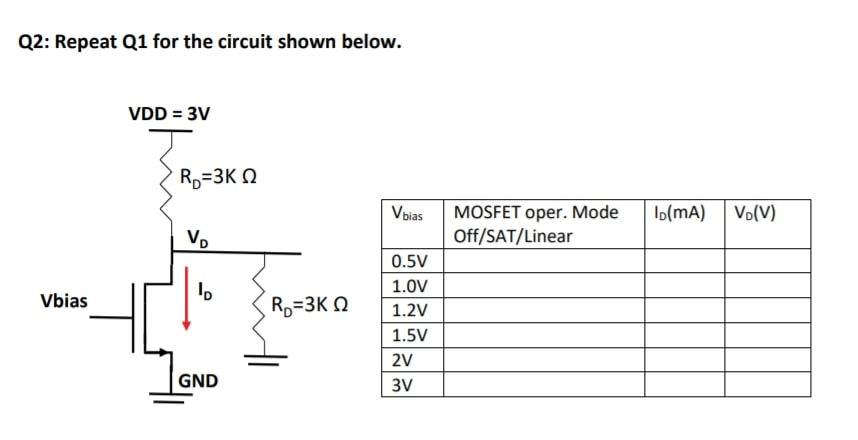
\includegraphics{./image/act1_p2.jpg}
\caption{Problem-2}
\end{figure}

\begin{longtable}[]{@{}llll@{}}
\toprule
\(V_{bias}\) & MOSFET Operation Mode & \(I_D\) (mA) & \(V_D\)
(V)\tabularnewline
\midrule
\endhead
0.5 & OFF & 0 & 1.5\tabularnewline
1.0 & SAT & .175 & 1.23\tabularnewline
1.2 & SAT & .377 & .93\tabularnewline
1.5 & LINEAR & .650 & .514\tabularnewline
2.0 & LINEAR & .783 & .325\tabularnewline
3.0 & LINEAR & .869 & .196\tabularnewline
\bottomrule
\end{longtable}

    \begin{tcolorbox}[breakable, size=fbox, boxrule=1pt, pad at break*=1mm,colback=cellbackground, colframe=cellborder]
\prompt{In}{incolor}{58}{\boxspacing}
\begin{Verbatim}[commandchars=\\\{\}]
\PY{k+kn}{import} \PY{n+nn}{numpy} \PY{k}{as} \PY{n+nn}{np}

\PY{c+c1}{\PYZsh{} Saturation}
\PY{k}{def} \PY{n+nf}{drain\PYZus{}voltage} \PY{p}{(}\PY{n}{VCC}\PY{o}{=}\PY{k+kc}{None}\PY{p}{,} \PY{n}{ID}\PY{o}{=}\PY{k+kc}{None}\PY{p}{,} \PY{n}{RD1}\PY{o}{=}\PY{k+kc}{None}\PY{p}{,} \PY{n}{RD2}\PY{o}{=}\PY{k+kc}{None}\PY{p}{,} \PY{n}{VGS}\PY{o}{=}\PY{k+kc}{None}\PY{p}{,} \PY{n}{VTH}\PY{o}{=}\PY{k+kc}{None}\PY{p}{,} \PY{n}{VDS}\PY{o}{=}\PY{k+kc}{None}\PY{p}{,} \PY{n}{fet\PYZus{}mode}\PY{o}{=}\PY{l+s+s1}{\PYZsq{}}\PY{l+s+s1}{\PYZsq{}}\PY{p}{)}\PY{p}{:}
    \PY{k}{if} \PY{n}{fet\PYZus{}mode}\PY{o}{==}\PY{l+s+s2}{\PYZdq{}}\PY{l+s+s2}{sat}\PY{l+s+s2}{\PYZdq{}}\PY{p}{:}
        \PY{n}{VDS} \PY{o}{=} \PY{n}{parallel\PYZus{}resistance}\PY{p}{(}\PY{n}{R1}\PY{o}{=}\PY{n}{RD1}\PY{p}{,} \PY{n}{R2}\PY{o}{=}\PY{n}{RD2}\PY{p}{)}\PY{o}{*}\PY{p}{(}\PY{n}{VCC}\PY{o}{/}\PY{n}{RD1}\PY{o}{\PYZhy{}}\PY{n}{ID}\PY{p}{)}
        \PY{n}{mode\PYZus{}true} \PY{o}{=} \PY{n}{VDS} \PY{o}{\PYZgt{}} \PY{p}{(}\PY{n}{VGS}\PY{o}{\PYZhy{}}\PY{n}{VTH}\PY{p}{)}
        \PY{n+nb}{print}\PY{p}{(}\PY{l+s+s2}{\PYZdq{}}\PY{l+s+s2}{VDS = }\PY{l+s+si}{\PYZob{}\PYZcb{}}\PY{l+s+s2}{ V, the assumption is }\PY{l+s+si}{\PYZob{}\PYZcb{}}\PY{l+s+s2}{.}\PY{l+s+s2}{\PYZdq{}}\PY{o}{.}\PY{n}{format}\PY{p}{(}\PY{n}{VDS}\PY{p}{,} \PY{n}{mode\PYZus{}true}\PY{p}{)}\PY{p}{)}
        \PY{k}{return} \PY{n}{VDS}
    \PY{k}{elif} \PY{n}{fet\PYZus{}mode}\PY{o}{==}\PY{l+s+s1}{\PYZsq{}}\PY{l+s+s1}{triode}\PY{l+s+s1}{\PYZsq{}}\PY{p}{:}
        \PY{n}{mode\PYZus{}true} \PY{o}{=} \PY{n}{VDS} \PY{o}{\PYZlt{}} \PY{p}{(}\PY{n}{VGS}\PY{o}{\PYZhy{}}\PY{n}{VTH}\PY{p}{)}
        \PY{n+nb}{print}\PY{p}{(}\PY{l+s+s2}{\PYZdq{}}\PY{l+s+s2}{VDS = }\PY{l+s+si}{\PYZob{}\PYZcb{}}\PY{l+s+s2}{ V, the assumption is }\PY{l+s+si}{\PYZob{}\PYZcb{}}\PY{l+s+s2}{.}\PY{l+s+s2}{\PYZdq{}}\PY{o}{.}\PY{n}{format}\PY{p}{(}\PY{n}{VDS}\PY{p}{,} \PY{n}{mode\PYZus{}true}\PY{p}{)}\PY{p}{)}
        \PY{k}{return} \PY{n}{VDS}
    \PY{k}{return} \PY{k+kc}{None}
\PY{k}{def} \PY{n+nf}{parallel\PYZus{}resistance} \PY{p}{(}\PY{n}{R1}\PY{p}{,} \PY{n}{R2}\PY{p}{)}\PY{p}{:}
    \PY{k}{return} \PY{n}{R1}\PY{o}{*}\PY{n}{R2}\PY{o}{/}\PY{p}{(}\PY{n}{R1}\PY{o}{+}\PY{n}{R2}\PY{p}{)}

\PY{c+c1}{\PYZsh{} Triode}
\PY{k}{def} \PY{n+nf}{quadratic\PYZus{}formula} \PY{p}{(}\PY{n}{a}\PY{p}{,}\PY{n}{b}\PY{p}{,}\PY{n}{c}\PY{p}{)}\PY{p}{:}
    \PY{n}{d} \PY{o}{=} \PY{p}{(}\PY{n}{b}\PY{o}{*}\PY{o}{*}\PY{l+m+mi}{2}\PY{p}{)} \PY{o}{\PYZhy{}} \PY{p}{(}\PY{l+m+mi}{4}\PY{o}{*}\PY{n}{a}\PY{o}{*}\PY{n}{c}\PY{p}{)}  
    \PY{n}{sol1} \PY{o}{=} \PY{p}{(}\PY{o}{\PYZhy{}}\PY{n}{b}\PY{o}{\PYZhy{}}\PY{n}{cmath}\PY{o}{.}\PY{n}{sqrt}\PY{p}{(}\PY{n}{d}\PY{p}{)}\PY{p}{)}\PY{o}{/}\PY{p}{(}\PY{l+m+mi}{2}\PY{o}{*}\PY{n}{a}\PY{p}{)}  
    \PY{n}{sol2} \PY{o}{=} \PY{p}{(}\PY{o}{\PYZhy{}}\PY{n}{b}\PY{o}{+}\PY{n}{cmath}\PY{o}{.}\PY{n}{sqrt}\PY{p}{(}\PY{n}{d}\PY{p}{)}\PY{p}{)}\PY{o}{/}\PY{p}{(}\PY{l+m+mi}{2}\PY{o}{*}\PY{n}{a}\PY{p}{)}  
    \PY{n+nb}{print}\PY{p}{(}\PY{l+s+s1}{\PYZsq{}}\PY{l+s+s1}{The solution are }\PY{l+s+si}{\PYZob{}0\PYZcb{}}\PY{l+s+s1}{ and }\PY{l+s+si}{\PYZob{}1\PYZcb{}}\PY{l+s+s1}{\PYZsq{}}\PY{o}{.}\PY{n}{format}\PY{p}{(}\PY{n}{sol1}\PY{p}{,}\PY{n}{sol2}\PY{p}{)}\PY{p}{)}
    \PY{k}{return} \PY{p}{[}\PY{n}{sol1}\PY{p}{,} \PY{n}{sol2}\PY{p}{]}
\PY{k}{def} \PY{n+nf}{current\PYZus{}post\PYZus{}quad} \PY{p}{(}\PY{n}{VCC}\PY{p}{,} \PY{n}{VDS}\PY{p}{,} \PY{n}{RD1}\PY{p}{,}\PY{n}{RD2}\PY{p}{)}\PY{p}{:}
    \PY{n}{ID} \PY{o}{=} \PY{n}{VCC}\PY{o}{/}\PY{n}{RD1}\PY{o}{\PYZhy{}}\PY{n}{VDS}\PY{o}{*}\PY{p}{(}\PY{n}{parallel\PYZus{}resistance}\PY{p}{(}\PY{n}{R1}\PY{o}{=}\PY{n}{RD1}\PY{p}{,}\PY{n}{R2}\PY{o}{=}\PY{n}{RD2}\PY{p}{)}\PY{o}{*}\PY{o}{*}\PY{p}{(}\PY{o}{\PYZhy{}}\PY{l+m+mi}{1}\PY{p}{)}\PY{p}{)}
    \PY{n+nb}{print}\PY{p}{(}\PY{l+s+s1}{\PYZsq{}}\PY{l+s+s1}{ID = }\PY{l+s+si}{\PYZob{}\PYZcb{}}\PY{l+s+s1}{ A}\PY{l+s+s1}{\PYZsq{}}\PY{o}{.}\PY{n}{format}\PY{p}{(}\PY{n}{ID}\PY{p}{)}\PY{p}{)}
    \PY{k}{return} \PY{n}{ID}
\end{Verbatim}
\end{tcolorbox}

    \begin{tcolorbox}[breakable, size=fbox, boxrule=1pt, pad at break*=1mm,colback=cellbackground, colframe=cellborder]
\prompt{In}{incolor}{42}{\boxspacing}
\begin{Verbatim}[commandchars=\\\{\}]
\PY{n}{W} \PY{o}{=} \PY{l+m+mf}{3.5}
\PY{n}{L} \PY{o}{=} \PY{l+m+mf}{0.35}
\PY{n}{K\PYZus{}prime} \PY{o}{=} \PY{l+m+mi}{190}\PY{o}{*}\PY{l+m+mi}{10}\PY{o}{*}\PY{o}{*}\PY{p}{(}\PY{o}{\PYZhy{}}\PY{l+m+mi}{6}\PY{p}{)}
\PY{n}{Kn} \PY{o}{=} \PY{n}{W}\PY{o}{/}\PY{n}{L}\PY{o}{*}\PY{n}{K\PYZus{}prime}
\PY{n}{VGS} \PY{o}{=} \PY{l+m+mi}{1}
\PY{n}{VTH} \PY{o}{=} \PY{l+m+mf}{0.57}
\PY{n}{ID} \PY{o}{=} \PY{n}{saturation\PYZus{}current}\PY{p}{(}\PY{n}{VGS}\PY{p}{,}\PY{n}{VTH}\PY{p}{,}\PY{n}{Kn}\PY{p}{,}\PY{n}{fet\PYZus{}mode}\PY{o}{=}\PY{l+s+s1}{\PYZsq{}}\PY{l+s+s1}{sat}\PY{l+s+s1}{\PYZsq{}}\PY{p}{)}
\PY{n}{VCC} \PY{o}{=} \PY{l+m+mi}{3}
\PY{n}{RD}\PY{o}{=}\PY{l+m+mi}{3000}
\PY{c+c1}{\PYZsh{}verification}
\PY{n}{drain\PYZus{}voltage} \PY{p}{(}\PY{n}{VCC}\PY{o}{=}\PY{n}{VCC}\PY{p}{,} \PY{n}{ID}\PY{o}{=}\PY{n}{ID}\PY{p}{,} \PY{n}{RD1}\PY{o}{=}\PY{n}{RD}\PY{p}{,} \PY{n}{RD2}\PY{o}{=}\PY{n}{RD}\PY{p}{,}\PYZbs{}
               \PY{n}{VGS}\PY{o}{=}\PY{n}{VGS}\PY{p}{,}\PY{n}{VTH}\PY{o}{=}\PY{n}{VTH}\PY{p}{,} \PY{n}{fet\PYZus{}mode}\PY{o}{=}\PY{l+s+s1}{\PYZsq{}}\PY{l+s+s1}{sat}\PY{l+s+s1}{\PYZsq{}}\PY{p}{)}
\end{Verbatim}
\end{tcolorbox}

    \begin{Verbatim}[commandchars=\\\{\}]
The saturation current is: 0.175655 mA
VDS = 1.2365175 V, the assumption is True.
    \end{Verbatim}

            \begin{tcolorbox}[breakable, size=fbox, boxrule=.5pt, pad at break*=1mm, opacityfill=0]
\prompt{Out}{outcolor}{42}{\boxspacing}
\begin{Verbatim}[commandchars=\\\{\}]
1.2365175
\end{Verbatim}
\end{tcolorbox}
        
    \begin{tcolorbox}[breakable, size=fbox, boxrule=1pt, pad at break*=1mm,colback=cellbackground, colframe=cellborder]
\prompt{In}{incolor}{43}{\boxspacing}
\begin{Verbatim}[commandchars=\\\{\}]
\PY{n}{W} \PY{o}{=} \PY{l+m+mf}{3.5}
\PY{n}{L} \PY{o}{=} \PY{l+m+mf}{0.35}
\PY{n}{K\PYZus{}prime} \PY{o}{=} \PY{l+m+mi}{190}\PY{o}{*}\PY{l+m+mi}{10}\PY{o}{*}\PY{o}{*}\PY{p}{(}\PY{o}{\PYZhy{}}\PY{l+m+mi}{6}\PY{p}{)}
\PY{n}{Kn} \PY{o}{=} \PY{n}{W}\PY{o}{/}\PY{n}{L}\PY{o}{*}\PY{n}{K\PYZus{}prime}
\PY{n}{VGS} \PY{o}{=} \PY{l+m+mf}{1.2}
\PY{n}{VTH} \PY{o}{=} \PY{l+m+mf}{0.57}
\PY{n}{ID} \PY{o}{=} \PY{n}{saturation\PYZus{}current}\PY{p}{(}\PY{n}{VGS}\PY{p}{,}\PY{n}{VTH}\PY{p}{,}\PY{n}{Kn}\PY{p}{,}\PY{n}{fet\PYZus{}mode}\PY{o}{=}\PY{l+s+s1}{\PYZsq{}}\PY{l+s+s1}{sat}\PY{l+s+s1}{\PYZsq{}}\PY{p}{)}
\PY{n}{VCC} \PY{o}{=} \PY{l+m+mi}{3}
\PY{n}{RD}\PY{o}{=}\PY{l+m+mi}{3000}
\PY{c+c1}{\PYZsh{}verification}
\PY{n}{drain\PYZus{}voltage} \PY{p}{(}\PY{n}{VCC}\PY{o}{=}\PY{n}{VCC}\PY{p}{,} \PY{n}{ID}\PY{o}{=}\PY{n}{ID}\PY{p}{,} \PY{n}{RD1}\PY{o}{=}\PY{n}{RD}\PY{p}{,} \PY{n}{RD2}\PY{o}{=}\PY{n}{RD}\PY{p}{,}\PYZbs{}
               \PY{n}{VGS}\PY{o}{=}\PY{n}{VGS}\PY{p}{,}\PY{n}{VTH}\PY{o}{=}\PY{n}{VTH}\PY{p}{,} \PY{n}{fet\PYZus{}mode}\PY{o}{=}\PY{l+s+s1}{\PYZsq{}}\PY{l+s+s1}{sat}\PY{l+s+s1}{\PYZsq{}}\PY{p}{)}
\end{Verbatim}
\end{tcolorbox}

    \begin{Verbatim}[commandchars=\\\{\}]
The saturation current is: 0.377055 mA
VDS = 0.9344174999999999 V, the assumption is True.
    \end{Verbatim}

            \begin{tcolorbox}[breakable, size=fbox, boxrule=.5pt, pad at break*=1mm, opacityfill=0]
\prompt{Out}{outcolor}{43}{\boxspacing}
\begin{Verbatim}[commandchars=\\\{\}]
0.9344174999999999
\end{Verbatim}
\end{tcolorbox}
        
    \begin{tcolorbox}[breakable, size=fbox, boxrule=1pt, pad at break*=1mm,colback=cellbackground, colframe=cellborder]
\prompt{In}{incolor}{38}{\boxspacing}
\begin{Verbatim}[commandchars=\\\{\}]
\PY{n}{W} \PY{o}{=} \PY{l+m+mf}{3.5}
\PY{n}{L} \PY{o}{=} \PY{l+m+mf}{0.35}
\PY{n}{K\PYZus{}prime} \PY{o}{=} \PY{l+m+mi}{190}\PY{o}{*}\PY{l+m+mi}{10}\PY{o}{*}\PY{o}{*}\PY{p}{(}\PY{o}{\PYZhy{}}\PY{l+m+mi}{6}\PY{p}{)}
\PY{n}{Kn} \PY{o}{=} \PY{n}{W}\PY{o}{/}\PY{n}{L}\PY{o}{*}\PY{n}{K\PYZus{}prime}
\PY{n}{VGS} \PY{o}{=} \PY{l+m+mf}{1.5}
\PY{n}{VTH} \PY{o}{=} \PY{l+m+mf}{0.57}
\PY{n}{ID} \PY{o}{=} \PY{n}{saturation\PYZus{}current}\PY{p}{(}\PY{n}{VGS}\PY{p}{,}\PY{n}{VTH}\PY{p}{,}\PY{n}{Kn}\PY{p}{,}\PY{n}{fet\PYZus{}mode}\PY{o}{=}\PY{l+s+s1}{\PYZsq{}}\PY{l+s+s1}{sat}\PY{l+s+s1}{\PYZsq{}}\PY{p}{)}
\PY{n}{VCC} \PY{o}{=} \PY{l+m+mi}{3}
\PY{n}{RD1}\PY{o}{=}\PY{l+m+mi}{3000}
\PY{n}{RD2}\PY{o}{=}\PY{l+m+mi}{3000}
\PY{c+c1}{\PYZsh{}verification}
\PY{n}{drain\PYZus{}voltage} \PY{p}{(}\PY{n}{VCC}\PY{o}{=}\PY{n}{VCC}\PY{p}{,} \PY{n}{ID}\PY{o}{=}\PY{n}{ID}\PY{p}{,} \PY{n}{RD1}\PY{o}{=}\PY{n}{RD}\PY{p}{,} \PY{n}{RD2}\PY{o}{=}\PY{n}{RD}\PY{p}{,}\PYZbs{}
               \PY{n}{VGS}\PY{o}{=}\PY{n}{VGS}\PY{p}{,}\PY{n}{VTH}\PY{o}{=}\PY{n}{VTH}\PY{p}{,} \PY{n}{fet\PYZus{}mode}\PY{o}{=}\PY{l+s+s1}{\PYZsq{}}\PY{l+s+s1}{sat}\PY{l+s+s1}{\PYZsq{}}\PY{p}{)}

\PY{c+c1}{\PYZsh{} verification fail \PYZhy{}\PYZgt{} so it\PYZsq{}s triode}
\PY{c+c1}{\PYZsh{} VDS}
\PY{n}{a} \PY{o}{=} \PY{n}{Kn}\PY{o}{/}\PY{l+m+mi}{2}
\PY{n}{b} \PY{o}{=} \PY{o}{\PYZhy{}}\PY{l+m+mi}{1}\PY{o}{*}\PY{p}{(}\PY{n}{Kn}\PY{o}{*}\PY{p}{(}\PY{n}{VGS}\PY{o}{\PYZhy{}}\PY{n}{VTH}\PY{p}{)}\PY{o}{+}\PY{n}{parallel\PYZus{}resistance}\PY{p}{(}\PY{n}{R1}\PY{o}{=}\PY{n}{RD1}\PY{p}{,} \PY{n}{R2}\PY{o}{=}\PY{n}{RD2}\PY{p}{)}\PY{o}{*}\PY{o}{*}\PY{p}{(}\PY{o}{\PYZhy{}}\PY{l+m+mi}{1}\PY{p}{)}\PY{p}{)}
\PY{n}{c} \PY{o}{=} \PY{n}{VCC}\PY{o}{/}\PY{n}{RD1}
\PY{n}{Vd1}\PY{p}{,} \PY{n}{Vd2} \PY{o}{=} \PY{n}{quadratic\PYZus{}formula}\PY{p}{(}\PY{n}{a}\PY{o}{=}\PY{n}{a}\PY{p}{,}\PY{n}{b}\PY{o}{=}\PY{n}{b}\PY{p}{,}\PY{n}{c}\PY{o}{=}\PY{n}{c}\PY{p}{)}
\PY{n}{VDS} \PY{o}{=} \PY{n+nb}{min}\PY{p}{(}\PY{n+nb}{abs}\PY{p}{(}\PY{n}{Vd1}\PY{p}{)}\PY{p}{,}\PY{n+nb}{abs}\PY{p}{(}\PY{n}{Vd2}\PY{p}{)}\PY{p}{)}
\PY{n+nb}{print}\PY{p}{(}\PY{l+s+s1}{\PYZsq{}}\PY{l+s+s1}{The valid VDS here is: }\PY{l+s+si}{\PYZob{}\PYZcb{}}\PY{l+s+s1}{ V}\PY{l+s+s1}{\PYZsq{}}\PY{o}{.}\PY{n}{format}\PY{p}{(}\PY{n}{VDS}\PY{p}{)}\PY{p}{)}
\PY{c+c1}{\PYZsh{} ID}
\PY{n}{ID} \PY{o}{=} \PY{n}{current\PYZus{}post\PYZus{}quad}\PY{p}{(}\PY{n}{VCC}\PY{o}{=}\PY{n}{VCC}\PY{p}{,} \PY{n}{VDS}\PY{o}{=}\PY{n}{VDS}\PY{p}{,} \PY{n}{RD1}\PY{o}{=}\PY{n}{RD1}\PY{p}{,}\PY{n}{RD2}\PY{o}{=}\PY{n}{RD2}\PY{p}{)}
\end{Verbatim}
\end{tcolorbox}

    \begin{Verbatim}[commandchars=\\\{\}]
The saturation current is: 0.821655 mA
VDS = 0.2675175 V, the assumption is False.
The solution are (0.5140559592159103+0j) and (2.047698426749002+0j)
The valid VDS here is: 0.5140559592159103 V
ID = 0.0006572960271893932 A
    \end{Verbatim}

    \begin{tcolorbox}[breakable, size=fbox, boxrule=1pt, pad at break*=1mm,colback=cellbackground, colframe=cellborder]
\prompt{In}{incolor}{39}{\boxspacing}
\begin{Verbatim}[commandchars=\\\{\}]
\PY{n}{W} \PY{o}{=} \PY{l+m+mf}{3.5}
\PY{n}{L} \PY{o}{=} \PY{l+m+mf}{0.35}
\PY{n}{K\PYZus{}prime} \PY{o}{=} \PY{l+m+mi}{190}\PY{o}{*}\PY{l+m+mi}{10}\PY{o}{*}\PY{o}{*}\PY{p}{(}\PY{o}{\PYZhy{}}\PY{l+m+mi}{6}\PY{p}{)}
\PY{n}{Kn} \PY{o}{=} \PY{n}{W}\PY{o}{/}\PY{n}{L}\PY{o}{*}\PY{n}{K\PYZus{}prime}
\PY{n}{VGS} \PY{o}{=} \PY{l+m+mi}{2}
\PY{n}{VTH} \PY{o}{=} \PY{l+m+mf}{0.57}
\PY{n}{ID} \PY{o}{=} \PY{n}{saturation\PYZus{}current}\PY{p}{(}\PY{n}{VGS}\PY{p}{,}\PY{n}{VTH}\PY{p}{,}\PY{n}{Kn}\PY{p}{,}\PY{n}{fet\PYZus{}mode}\PY{o}{=}\PY{l+s+s1}{\PYZsq{}}\PY{l+s+s1}{sat}\PY{l+s+s1}{\PYZsq{}}\PY{p}{)}
\PY{n}{VCC} \PY{o}{=} \PY{l+m+mi}{3}
\PY{n}{RD1}\PY{o}{=}\PY{l+m+mi}{3000}
\PY{n}{RD2}\PY{o}{=}\PY{l+m+mi}{3000}
\PY{c+c1}{\PYZsh{}verification}
\PY{n}{drain\PYZus{}voltage} \PY{p}{(}\PY{n}{VCC}\PY{o}{=}\PY{n}{VCC}\PY{p}{,} \PY{n}{ID}\PY{o}{=}\PY{n}{ID}\PY{p}{,} \PY{n}{RD1}\PY{o}{=}\PY{n}{RD}\PY{p}{,} \PY{n}{RD2}\PY{o}{=}\PY{n}{RD}\PY{p}{,}\PYZbs{}
               \PY{n}{VGS}\PY{o}{=}\PY{n}{VGS}\PY{p}{,}\PY{n}{VTH}\PY{o}{=}\PY{n}{VTH}\PY{p}{,} \PY{n}{fet\PYZus{}mode}\PY{o}{=}\PY{l+s+s1}{\PYZsq{}}\PY{l+s+s1}{sat}\PY{l+s+s1}{\PYZsq{}}\PY{p}{)}

\PY{c+c1}{\PYZsh{} verification fail \PYZhy{}\PYZgt{} so it\PYZsq{}s triode}
\PY{c+c1}{\PYZsh{} VDS}
\PY{n}{a} \PY{o}{=} \PY{n}{Kn}\PY{o}{/}\PY{l+m+mi}{2}
\PY{n}{b} \PY{o}{=} \PY{o}{\PYZhy{}}\PY{l+m+mi}{1}\PY{o}{*}\PY{p}{(}\PY{n}{Kn}\PY{o}{*}\PY{p}{(}\PY{n}{VGS}\PY{o}{\PYZhy{}}\PY{n}{VTH}\PY{p}{)}\PY{o}{+}\PY{n}{parallel\PYZus{}resistance}\PY{p}{(}\PY{n}{R1}\PY{o}{=}\PY{n}{RD1}\PY{p}{,} \PY{n}{R2}\PY{o}{=}\PY{n}{RD2}\PY{p}{)}\PY{o}{*}\PY{o}{*}\PY{p}{(}\PY{o}{\PYZhy{}}\PY{l+m+mi}{1}\PY{p}{)}\PY{p}{)}
\PY{n}{c} \PY{o}{=} \PY{n}{VCC}\PY{o}{/}\PY{n}{RD1}
\PY{n}{Vd1}\PY{p}{,} \PY{n}{Vd2} \PY{o}{=} \PY{n}{quadratic\PYZus{}formula}\PY{p}{(}\PY{n}{a}\PY{o}{=}\PY{n}{a}\PY{p}{,}\PY{n}{b}\PY{o}{=}\PY{n}{b}\PY{p}{,}\PY{n}{c}\PY{o}{=}\PY{n}{c}\PY{p}{)}
\PY{n}{VDS} \PY{o}{=} \PY{n+nb}{min}\PY{p}{(}\PY{n+nb}{abs}\PY{p}{(}\PY{n}{Vd1}\PY{p}{)}\PY{p}{,}\PY{n+nb}{abs}\PY{p}{(}\PY{n}{Vd2}\PY{p}{)}\PY{p}{)}
\PY{n+nb}{print}\PY{p}{(}\PY{l+s+s1}{\PYZsq{}}\PY{l+s+s1}{The valid VDS here is: }\PY{l+s+si}{\PYZob{}\PYZcb{}}\PY{l+s+s1}{ V}\PY{l+s+s1}{\PYZsq{}}\PY{o}{.}\PY{n}{format}\PY{p}{(}\PY{n}{VDS}\PY{p}{)}\PY{p}{)}
\PY{c+c1}{\PYZsh{} ID}
\PY{n}{ID} \PY{o}{=} \PY{n}{current\PYZus{}post\PYZus{}quad}\PY{p}{(}\PY{n}{VCC}\PY{o}{=}\PY{n}{VCC}\PY{p}{,} \PY{n}{VDS}\PY{o}{=}\PY{n}{VDS}\PY{p}{,} \PY{n}{RD1}\PY{o}{=}\PY{n}{RD1}\PY{p}{,}\PY{n}{RD2}\PY{o}{=}\PY{n}{RD2}\PY{p}{)}
\end{Verbatim}
\end{tcolorbox}

    \begin{Verbatim}[commandchars=\\\{\}]
The saturation current is: 1.9426550000000005 mA
VDS = -1.4139825000000006 V, the assumption is False.
The solution are (0.3252357544620683+0j) and (3.236518631502844+0j)
The valid VDS here is: 0.3252357544620683 V
ID = 0.0007831761636919545 A
    \end{Verbatim}

    \begin{tcolorbox}[breakable, size=fbox, boxrule=1pt, pad at break*=1mm,colback=cellbackground, colframe=cellborder]
\prompt{In}{incolor}{40}{\boxspacing}
\begin{Verbatim}[commandchars=\\\{\}]
\PY{n}{W} \PY{o}{=} \PY{l+m+mf}{3.5}
\PY{n}{L} \PY{o}{=} \PY{l+m+mf}{0.35}
\PY{n}{K\PYZus{}prime} \PY{o}{=} \PY{l+m+mi}{190}\PY{o}{*}\PY{l+m+mi}{10}\PY{o}{*}\PY{o}{*}\PY{p}{(}\PY{o}{\PYZhy{}}\PY{l+m+mi}{6}\PY{p}{)}
\PY{n}{Kn} \PY{o}{=} \PY{n}{W}\PY{o}{/}\PY{n}{L}\PY{o}{*}\PY{n}{K\PYZus{}prime}
\PY{n}{VGS} \PY{o}{=} \PY{l+m+mi}{3}
\PY{n}{VTH} \PY{o}{=} \PY{l+m+mf}{0.57}
\PY{n}{ID} \PY{o}{=} \PY{n}{saturation\PYZus{}current}\PY{p}{(}\PY{n}{VGS}\PY{p}{,}\PY{n}{VTH}\PY{p}{,}\PY{n}{Kn}\PY{p}{,}\PY{n}{fet\PYZus{}mode}\PY{o}{=}\PY{l+s+s1}{\PYZsq{}}\PY{l+s+s1}{sat}\PY{l+s+s1}{\PYZsq{}}\PY{p}{)}
\PY{n}{VCC} \PY{o}{=} \PY{l+m+mi}{3}
\PY{n}{RD1}\PY{o}{=}\PY{l+m+mi}{3000}
\PY{n}{RD2}\PY{o}{=}\PY{l+m+mi}{3000}
\PY{c+c1}{\PYZsh{}verification}
\PY{n}{drain\PYZus{}voltage} \PY{p}{(}\PY{n}{VCC}\PY{o}{=}\PY{n}{VCC}\PY{p}{,} \PY{n}{ID}\PY{o}{=}\PY{n}{ID}\PY{p}{,} \PY{n}{RD1}\PY{o}{=}\PY{n}{RD}\PY{p}{,} \PY{n}{RD2}\PY{o}{=}\PY{n}{RD}\PY{p}{,}\PYZbs{}
               \PY{n}{VGS}\PY{o}{=}\PY{n}{VGS}\PY{p}{,}\PY{n}{VTH}\PY{o}{=}\PY{n}{VTH}\PY{p}{,} \PY{n}{fet\PYZus{}mode}\PY{o}{=}\PY{l+s+s1}{\PYZsq{}}\PY{l+s+s1}{sat}\PY{l+s+s1}{\PYZsq{}}\PY{p}{)}

\PY{c+c1}{\PYZsh{} verification fail \PYZhy{}\PYZgt{} so it\PYZsq{}s triode}
\PY{c+c1}{\PYZsh{} VDS}
\PY{n}{a} \PY{o}{=} \PY{n}{Kn}\PY{o}{/}\PY{l+m+mi}{2}
\PY{n}{b} \PY{o}{=} \PY{o}{\PYZhy{}}\PY{l+m+mi}{1}\PY{o}{*}\PY{p}{(}\PY{n}{Kn}\PY{o}{*}\PY{p}{(}\PY{n}{VGS}\PY{o}{\PYZhy{}}\PY{n}{VTH}\PY{p}{)}\PY{o}{+}\PY{n}{parallel\PYZus{}resistance}\PY{p}{(}\PY{n}{R1}\PY{o}{=}\PY{n}{RD1}\PY{p}{,} \PY{n}{R2}\PY{o}{=}\PY{n}{RD2}\PY{p}{)}\PY{o}{*}\PY{o}{*}\PY{p}{(}\PY{o}{\PYZhy{}}\PY{l+m+mi}{1}\PY{p}{)}\PY{p}{)}
\PY{n}{c} \PY{o}{=} \PY{n}{VCC}\PY{o}{/}\PY{n}{RD1}
\PY{n}{Vd1}\PY{p}{,} \PY{n}{Vd2} \PY{o}{=} \PY{n}{quadratic\PYZus{}formula}\PY{p}{(}\PY{n}{a}\PY{o}{=}\PY{n}{a}\PY{p}{,}\PY{n}{b}\PY{o}{=}\PY{n}{b}\PY{p}{,}\PY{n}{c}\PY{o}{=}\PY{n}{c}\PY{p}{)}
\PY{n}{VDS} \PY{o}{=} \PY{n+nb}{min}\PY{p}{(}\PY{n+nb}{abs}\PY{p}{(}\PY{n}{Vd1}\PY{p}{)}\PY{p}{,}\PY{n+nb}{abs}\PY{p}{(}\PY{n}{Vd2}\PY{p}{)}\PY{p}{)}
\PY{n+nb}{print}\PY{p}{(}\PY{l+s+s1}{\PYZsq{}}\PY{l+s+s1}{The valid VDS here is: }\PY{l+s+si}{\PYZob{}\PYZcb{}}\PY{l+s+s1}{ V}\PY{l+s+s1}{\PYZsq{}}\PY{o}{.}\PY{n}{format}\PY{p}{(}\PY{n}{VDS}\PY{p}{)}\PY{p}{)}
\PY{c+c1}{\PYZsh{} ID}
\PY{n}{ID} \PY{o}{=} \PY{n}{current\PYZus{}post\PYZus{}quad}\PY{p}{(}\PY{n}{VCC}\PY{o}{=}\PY{n}{VCC}\PY{p}{,} \PY{n}{VDS}\PY{o}{=}\PY{n}{VDS}\PY{p}{,} \PY{n}{RD1}\PY{o}{=}\PY{n}{RD1}\PY{p}{,}\PY{n}{RD2}\PY{o}{=}\PY{n}{RD2}\PY{p}{)}
\end{Verbatim}
\end{tcolorbox}

    \begin{Verbatim}[commandchars=\\\{\}]
The saturation current is: 5.609655 mA
VDS = -6.9144825 V, the assumption is False.
The solution are (0.19618255270043303+0j) and (5.365571833264481+0j)
The valid VDS here is: 0.19618255270043303 V
ID = 0.0008692116315330447 A
    \end{Verbatim}

    \begin{tcolorbox}[breakable, size=fbox, boxrule=1pt, pad at break*=1mm,colback=cellbackground, colframe=cellborder]
\prompt{In}{incolor}{62}{\boxspacing}
\begin{Verbatim}[commandchars=\\\{\}]
\PY{c+c1}{\PYZsh{} Problem: what is the drain voltage when MOSFET transition from SAT \PYZhy{}\PYZgt{} TRI?}
\PY{c+c1}{\PYZsh{} AKA: What VDS would be to make that happen? }
\PY{c+c1}{\PYZsh{} unknown: VGS, VDS, ID}
\PY{c+c1}{\PYZsh{} known: VDS = VGS + VTH, device in saturation.}

\PY{c+c1}{\PYZsh{} input parameter}
\PY{n}{VCC} \PY{o}{=} \PY{l+m+mi}{3}
\PY{n}{RD1}\PY{o}{=}\PY{l+m+mi}{3000}
\PY{n}{RD2}\PY{o}{=}\PY{l+m+mi}{3000}
\PY{n}{W} \PY{o}{=} \PY{l+m+mf}{3.5}
\PY{n}{L} \PY{o}{=} \PY{l+m+mf}{0.35}
\PY{n}{K\PYZus{}prime} \PY{o}{=} \PY{l+m+mi}{190}\PY{o}{*}\PY{l+m+mi}{10}\PY{o}{*}\PY{o}{*}\PY{p}{(}\PY{o}{\PYZhy{}}\PY{l+m+mi}{6}\PY{p}{)}
\PY{n}{Kn} \PY{o}{=} \PY{n}{W}\PY{o}{/}\PY{n}{L}\PY{o}{*}\PY{n}{K\PYZus{}prime}
\PY{n}{VTH} \PY{o}{=} \PY{l+m+mf}{0.57}
\PY{n+nb}{print}\PY{p}{(}\PY{l+s+s2}{\PYZdq{}}\PY{l+s+s2}{Find the point where device transition from saturation to linear region}\PY{l+s+se}{\PYZbs{}n}\PY{l+s+s2}{\PYZdq{}}\PY{p}{)}
\PY{n}{a} \PY{o}{=} \PY{n}{Kn}\PY{o}{/}\PY{l+m+mi}{2}
\PY{n}{b} \PY{o}{=} \PY{n}{parallel\PYZus{}resistance}\PY{p}{(}\PY{n}{R1}\PY{o}{=}\PY{n}{RD1}\PY{p}{,} \PY{n}{R2}\PY{o}{=}\PY{n}{RD2}\PY{p}{)}\PY{o}{*}\PY{o}{*}\PY{p}{(}\PY{o}{\PYZhy{}}\PY{l+m+mi}{1}\PY{p}{)}
\PY{n}{c} \PY{o}{=} \PY{o}{\PYZhy{}}\PY{n}{VCC}\PY{o}{/}\PY{n}{RD1}
\PY{n+nb}{print}\PY{p}{(}\PY{l+s+s2}{\PYZdq{}}\PY{l+s+s2}{This is the 2 possible VD value}\PY{l+s+s2}{\PYZdq{}}\PY{p}{)}
\PY{n}{Vd1}\PY{p}{,} \PY{n}{Vd2} \PY{o}{=} \PY{n}{quadratic\PYZus{}formula}\PY{p}{(}\PY{n}{a}\PY{o}{=}\PY{n}{a}\PY{p}{,}\PY{n}{b}\PY{o}{=}\PY{n}{b}\PY{p}{,}\PY{n}{c}\PY{o}{=}\PY{n}{c}\PY{p}{)}

\PY{c+c1}{\PYZsh{}answer}
\PY{n}{VDS} \PY{o}{=} \PY{n+nb}{abs}\PY{p}{(}\PY{n}{Vd2}\PY{p}{)}
\PY{n+nb}{print}\PY{p}{(}\PY{l+s+s2}{\PYZdq{}}\PY{l+s+s2}{This is the ID value from the valid VDS value}\PY{l+s+s2}{\PYZdq{}}\PY{p}{)}
\PY{n}{ID} \PY{o}{=} \PY{n}{current\PYZus{}post\PYZus{}quad}\PY{p}{(}\PY{n}{VCC}\PY{o}{=}\PY{n}{VCC}\PY{p}{,} \PY{n}{VDS}\PY{o}{=}\PY{n}{VDS}\PY{p}{,} \PY{n}{RD1}\PY{o}{=}\PY{n}{RD1}\PY{p}{,}\PY{n}{RD2}\PY{o}{=}\PY{n}{RD2}\PY{p}{)}
\PY{n}{VGS} \PY{o}{=} \PY{n}{VDS} \PY{o}{+} \PY{n}{VTH}

\PY{c+c1}{\PYZsh{}output}
\PY{n+nb}{print}\PY{p}{(}\PY{l+s+s2}{\PYZdq{}}\PY{l+s+s2}{VDS would be about: }\PY{l+s+si}{\PYZob{}\PYZcb{}}\PY{l+s+s2}{ V}\PY{l+s+s2}{\PYZdq{}}\PY{o}{.}\PY{n}{format}\PY{p}{(}\PY{n}{Vd2}\PY{p}{)}\PY{p}{)} \PY{c+c1}{\PYZsh{}the positive digit one}
\PY{n+nb}{print}\PY{p}{(}\PY{l+s+s2}{\PYZdq{}}\PY{l+s+s2}{ID would be about: }\PY{l+s+si}{\PYZob{}\PYZcb{}}\PY{l+s+s2}{ A}\PY{l+s+s2}{\PYZdq{}}\PY{o}{.}\PY{n}{format}\PY{p}{(}\PY{n}{ID}\PY{p}{)}\PY{p}{)}
\PY{n+nb}{print}\PY{p}{(}\PY{l+s+s2}{\PYZdq{}}\PY{l+s+s2}{VGS would be about: }\PY{l+s+si}{\PYZob{}\PYZcb{}}\PY{l+s+s2}{ V}\PY{l+s+s2}{\PYZdq{}}\PY{o}{.}\PY{n}{format}\PY{p}{(}\PY{n}{VGS}\PY{p}{)}\PY{p}{)}
\end{Verbatim}
\end{tcolorbox}

    \begin{Verbatim}[commandchars=\\\{\}]
Find the point where device transition from saturation to linear region

This is the 2 possible VD value
The solution are (-1.4351955887973646+0j) and (0.7334412028324524+0j)
This is the ID value from the valid VDS value
ID = 0.0005110391981116984 A
VDS would be about: (0.7334412028324524+0j) V
ID would be about: 0.0005110391981116984 A
VGS would be about: 1.3034412028324525 V
    \end{Verbatim}

    \begin{tcolorbox}[breakable, size=fbox, boxrule=1pt, pad at break*=1mm,colback=cellbackground, colframe=cellborder]
\prompt{In}{incolor}{47}{\boxspacing}
\begin{Verbatim}[commandchars=\\\{\}]
\PY{n}{VGS} \PY{o}{=} \PY{p}{[}\PY{l+m+mf}{0.5}\PY{p}{,} \PY{l+m+mi}{1}\PY{p}{,} \PY{l+m+mf}{1.2}\PY{p}{,} \PY{l+m+mf}{1.303}\PY{p}{,} \PY{l+m+mf}{1.5}\PY{p}{,} \PY{l+m+mi}{2}\PY{p}{,} \PY{l+m+mi}{3}\PY{p}{]}
\PY{n}{ID} \PY{o}{=} \PY{p}{[}\PY{l+m+mi}{0}\PY{p}{,}\PY{o}{.}\PY{l+m+mi}{175}\PY{p}{,}\PY{o}{.}\PY{l+m+mi}{377}\PY{p}{,}\PY{l+m+mf}{0.511}\PY{p}{,}\PY{o}{.}\PY{l+m+mi}{65}\PY{p}{,}\PY{o}{.}\PY{l+m+mi}{783}\PY{p}{,}\PY{o}{.}\PY{l+m+mi}{869}\PY{p}{]}
\PY{n}{VD} \PY{o}{=} \PY{p}{[}\PY{l+m+mf}{1.5}\PY{p}{,}\PY{l+m+mf}{1.23}\PY{p}{,}\PY{l+m+mf}{0.93}\PY{p}{,}\PY{o}{.}\PY{l+m+mi}{733}\PY{p}{,}\PY{o}{.}\PY{l+m+mi}{51}\PY{p}{,}\PY{o}{.}\PY{l+m+mi}{325}\PY{p}{,}\PY{o}{.}\PY{l+m+mi}{196}\PY{p}{]}

\PY{c+c1}{\PYZsh{} ID vs. VGS}
\PY{n}{plot\PYZus{}point}\PY{p}{(}\PY{n}{t}\PY{o}{=}\PY{n}{VGS}\PY{p}{,} \PY{n}{data}\PY{o}{=}\PY{n}{ID}\PY{p}{,} \PY{n}{xlabel} \PY{o}{=} \PY{l+s+s1}{\PYZsq{}}\PY{l+s+s1}{VG (V)}\PY{l+s+s1}{\PYZsq{}}\PY{p}{,} \PY{n}{ylabel} \PY{o}{=} \PY{l+s+s1}{\PYZsq{}}\PY{l+s+s1}{Drain Current (mA)}\PY{l+s+s1}{\PYZsq{}}\PY{p}{,} \PY{n}{title} \PY{o}{=} \PY{l+s+s1}{\PYZsq{}}\PY{l+s+s1}{ID vs. VG}\PY{l+s+s1}{\PYZsq{}}\PY{p}{)}
\PY{c+c1}{\PYZsh{} VD vs. VGS}
\PY{n}{plot\PYZus{}point}\PY{p}{(}\PY{n}{t}\PY{o}{=}\PY{n}{VGS}\PY{p}{,} \PY{n}{data}\PY{o}{=}\PY{n}{VD}\PY{p}{,} \PY{n}{xlabel} \PY{o}{=} \PY{l+s+s1}{\PYZsq{}}\PY{l+s+s1}{VG (V)}\PY{l+s+s1}{\PYZsq{}}\PY{p}{,} \PY{n}{ylabel} \PY{o}{=} \PY{l+s+s1}{\PYZsq{}}\PY{l+s+s1}{Drain Voltage (V)}\PY{l+s+s1}{\PYZsq{}}\PY{p}{,} \PY{n}{title} \PY{o}{=} \PY{l+s+s1}{\PYZsq{}}\PY{l+s+s1}{VD vs. VG}\PY{l+s+s1}{\PYZsq{}}\PY{p}{)}
\end{Verbatim}
\end{tcolorbox}

    \begin{center}
    \adjustimage{max size={0.9\linewidth}{0.9\paperheight}}{output_20_0.png}
    \end{center}
    { \hspace*{\fill} \\}
    
    \begin{center}
    \adjustimage{max size={0.9\linewidth}{0.9\paperheight}}{output_20_1.png}
    \end{center}
    { \hspace*{\fill} \\}
    
    \hypertarget{problem-3}{%
\subsubsection{Problem 3}\label{problem-3}}

\begin{figure}
\centering
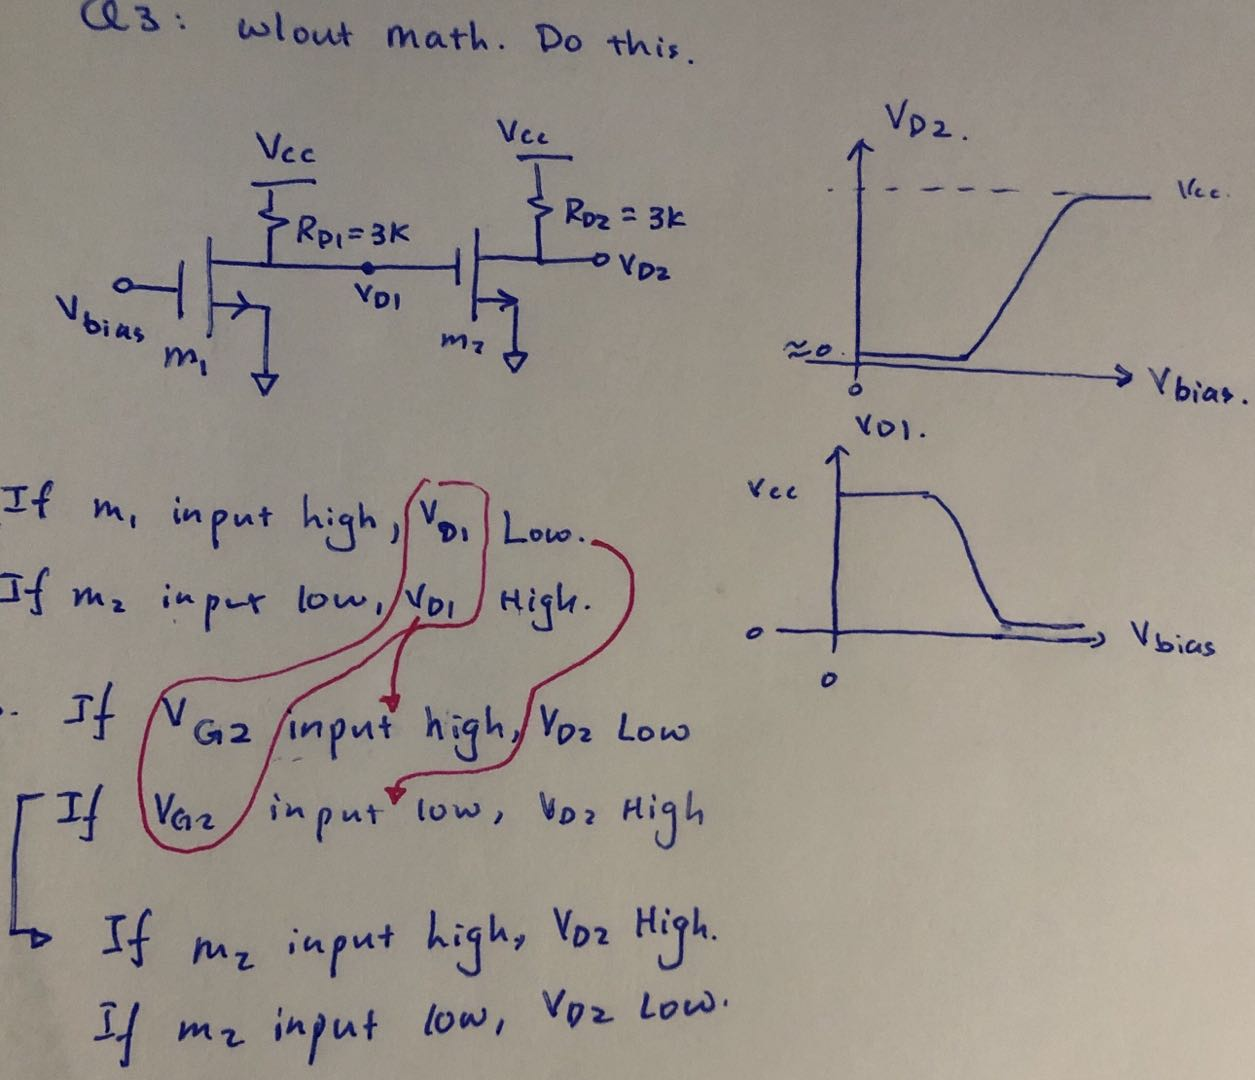
\includegraphics{./image/Q3-sol.jpg}
\caption{Problem-3}
\end{figure}

    \hypertarget{problem-4-part-1}{%
\subsubsection{Problem 4, part 1}\label{problem-4-part-1}}

\begin{figure}
\centering
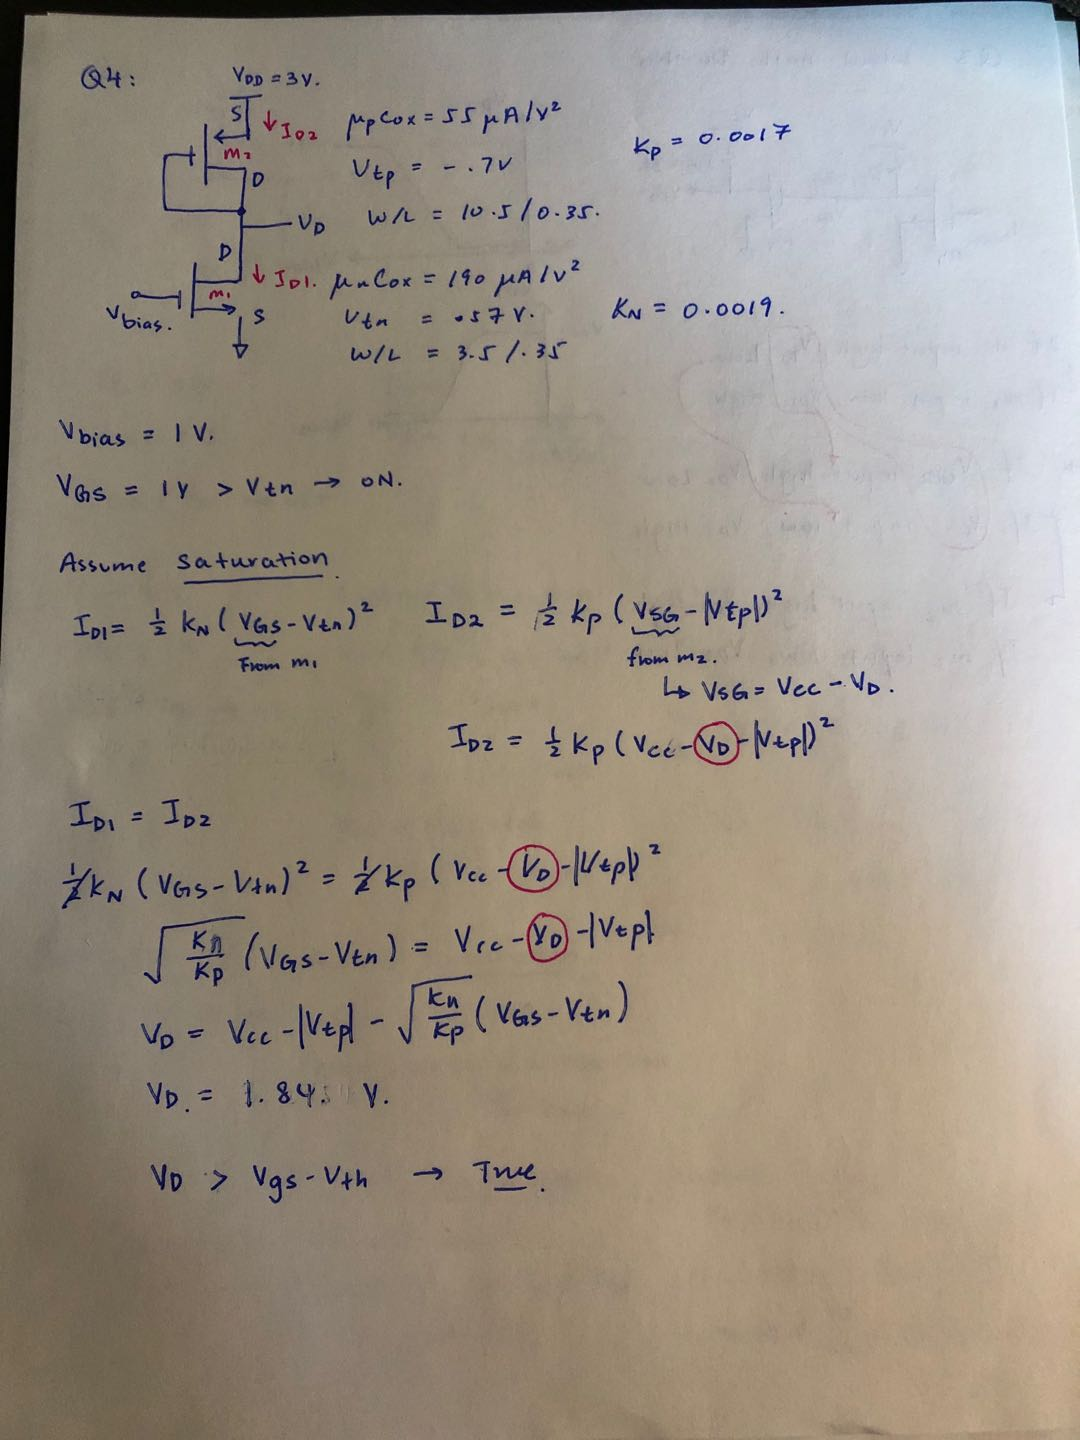
\includegraphics{./image/Q4-sol.jpg}
\caption{Problem-4}
\end{figure}

    \hypertarget{problem-4-part-2}{%
\subsubsection{Problem 4 , part 2}\label{problem-4-part-2}}

\begin{figure}
\centering
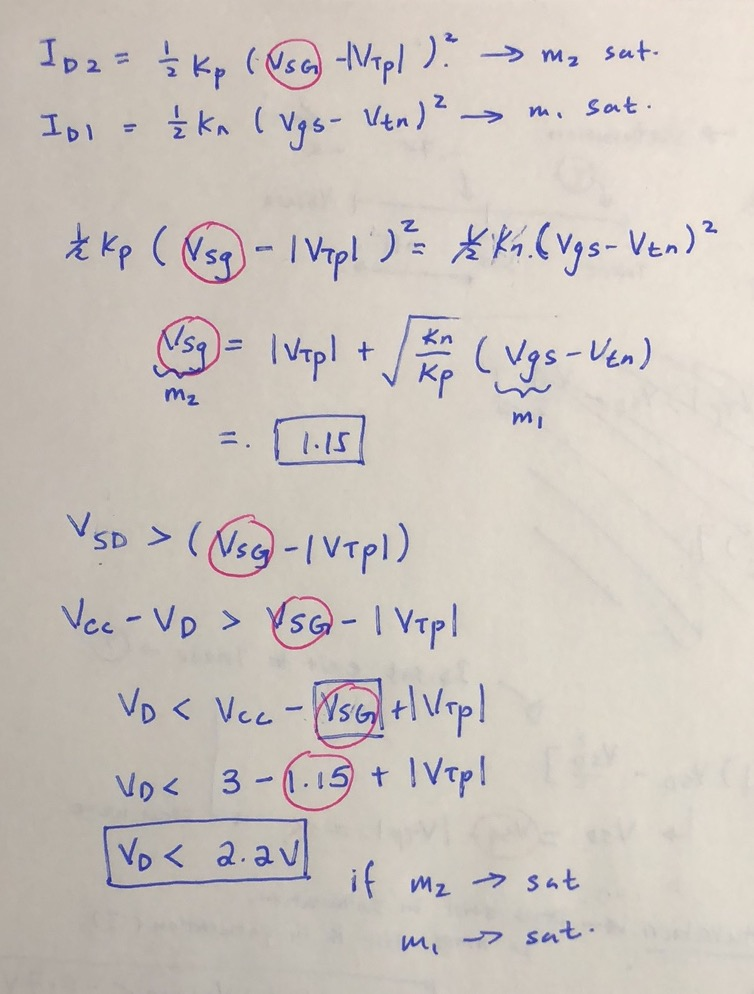
\includegraphics{./image/Q4-part2-sol.jpg}
\caption{Problem-4}
\end{figure}

    \hypertarget{problem-5}{%
\subsubsection{Problem 5}\label{problem-5}}

\begin{figure}
\centering
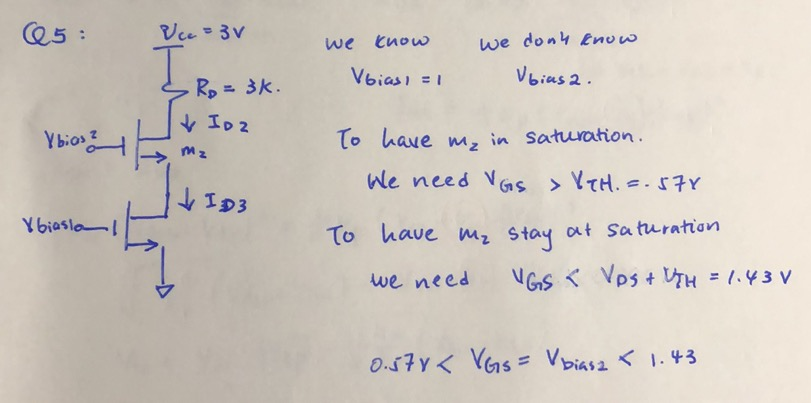
\includegraphics{./image/Q5-sol.jpg}
\caption{Problem-5}
\end{figure}


    % Add a bibliography block to the postdoc
    
    
    
\end{document}
